\chapter{Kryptologie}\label{ch:Kryptologie}

\lstset{style=Python}

\section{Einführung}\label{sec:intro}

Alice möchte Bob eine wichtige Nachricht zukommen lassen, beispielsweise zu einem gesundheitlichen Problem oder um ihre Bankkontoverbindung mit Bob zu teilen. Da das Internet jedoch eine \textit{offene} und somit (grundsätzlich) unsichere Technologie ist, kann jedermann jede Nachricht mitlesen. Somit könnte eine bösartige Person, wie beispielsweise Eve, die Nachricht abhören, um sich Zugriff auf die Gesundheitsdaten oder das Bankkonto von Alice zu verschaffen.

Damit dies nicht passieren kann, muss Alice ihre Nachricht so verschlüsseln, dass nur Bob sie lesen kann. Dieses Problem hat sich bereits in der Antike (und vermutlich noch vorher gestellt) und entspricht einem grundsätzlichen, menschlichen Bedürfnis: Wie kann ein Feldherr seinen Soldaten Anweisungen geben, ohne dass der Gegner mithört? Oder, um eine andere Situation aufzugreifen: Wie können Sie sich mit Ihren Geschwistern austauschen, ohne dass Ihre Eltern verstehen, worum es geht?

In der Informatik spricht man hier davon, dass Alice aus ihrem \enquote{Klartext}, also dem für alle Menschen verständlichen Text, einen \enquote{Kryptotext} macht, also einen Text, den nur Bob entschlüsseln kann, d.h., nur Bob weiss, wie man aus diesem Text wieder einen verständlichen Text macht. Hierzu muss man sich auf eine Verschlüsselungsmethode einigen. In der Informatik spricht man hierbei von einem \textbf{Verschlüsselungs-Algorithmus} und \textbf{Entschlüsselungs-Algorithmus}. Die Methode, um eine Nachricht zu verschlüsseln, so dass sie für Dritte unlesbar ist, wird häufig auch \enquote{\textbf{Schlüssel}} genannt, und das Verfahren, um eine Nachricht unlesbar zu machen \enquote{Verschlüsselung} oder \enquote{Chiffrierung}. Im Allgemeinen wird der Bereich der Informatik, der sich mit Ver- und Entschlüsselung befasst, \enquote{Kryptografie} genannt und die verschiedenen Algorithmen und Ansätze werden häufig als \enquote{Kryptosysteme} bezeichnet.
%
% \begin{figure}[H]
%     \centering
%     \begin{tikzpicture}[mylabel/.style={text width=20mm, align=center},scale=0.8, every node/.style={scale=0.8}]
%     \node[alice, minimum width=1.5cm, 
%         label={[mylabel, anchor=west]north east:{}}, 
%         label={[mylabel, anchor=east]north west:{\textcolor{Blue}{Klartext} $\big\downarrow\text{\tiny (Chiffrierung)}$\\
%         \textcolor{Red}{Kryptotext}}}] (alice) {Alice (Sender)};
%     \node[bob, minimum width=1.5cm, right=5cm of alice, mirrored,
%         label={[mylabel, anchor=east]north west:{}}, 
%         label={[mylabel, anchor=west]north east:{\textcolor{Red}{Kryptotext} $\big\downarrow\text{\tiny (Dechiffrierung)}$\\
%         \textcolor{Blue}{Klartext}}}] (bob) {Bob (Empfänger)};
%     
%     \draw[->, thick, black] ([yshift=0mm]alice.east) coordinate(aux-a)-- coordinate[near start] (aux) node[above, text width=3cm, align=center]{Übermittlung über unsicheren Kanal e.g. Internet, Telefonie \\
%     \textcolor{Red}{Kryptotext}} (aux-a-|bob.west);
%
%     \node[devil, minimum width=1.5cm, below right=13mm and 1.6cm of alice] (eve) {Eve (Gegner / Abhörer)};
%     \draw[<-, gray] (eve)--(aux) node[midway,right]{abhören};
%     \end{tikzpicture}
%     \caption{Dieses Schema zeigt die Kommunikation zwischen Alice (Sender) und Bob (Empfänger).}
%     \label{fig:schemaGeheimtext}
% \end{figure}
% \clearpage
%
% \section{Geheimschriften}
% \section{Kryptosysteme}
\begin{figure}[H]
	\centering
	\begin{tikzpicture}[mylabel/.style={text width=20mm, align=center},scale=0.8, every node/.style={scale=0.8}]
		\node[alice, minimum width=1.5cm,
		label={[mylabel, anchor=west]north east:{}},
		label={[mylabel, anchor=east]north west:{\textcolor{Blue}{(Klartext, Schlüssel)} $\big\downarrow\text{\tiny (Verschlüsselung)}$\\
		\textcolor{Red}{Kryptotext}}}] (alice) {Alice (Sender)};
		\node[bob, minimum width=1.5cm, right=5cm of alice, mirrored,
		label={[mylabel, anchor=east]north west:{}},
		label={[mylabel, anchor=west]north east:{\textcolor{Red}{(Kryptotext, Schlüssel)} $\big\downarrow\text{\tiny (Entschlüsselung)}$\\
		\textcolor{Blue}{Klartext}}}] (bob) {Bob (Empfänger)};

		\draw[->, thick, black] ([yshift=0mm]alice.east) coordinate(aux-a)-- coordinate[near start] (aux) node[above, text width=3cm, align=center]{Übermittlung über unsicheren Kanal e.g. Internet, Telefonie \\
				\textcolor{Red}{Kryptotext}} (aux-a-|bob.west);

		\node[devil, minimum width=1.5cm, below right=13mm and 1.6cm of alice] (eve) {Eve (Gegner / Abhörer)};
		\draw[<-, gray] (eve)--(aux) node[midway,right]{abhören};
	\end{tikzpicture}
	\caption{Dieses Schema zeigt die Kommunikation zwischen Alice (Sender) und Bob (Empfänger) unter Verwendung eines Kryptosystems.}
	\label{fig:schemaGeheimtext}
\end{figure}

Im Folgenden setzen wir uns zuerst mit einigen grundlegenden Verschlüsselungs-Methoden auseinander, um zu verstehen, was ein sicheres Kryptosystem auszeichnet. Der niederländische Kryptologe und Linguist Auguste Kerckhoffs stellte im Jahr 1883 sechs Grundsätze für sichere Verschlüsselungsverfahren auf:

\begin{figure}[H]
	\centering
	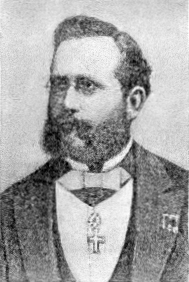
\includegraphics[width=0.3\linewidth]{Grundlagen_Info/03_Kryptologie/Figures/kerckhoffs}
	\caption{Auguste Kerckhoffs (1835-1903)}
	\label{fig:kerckhoffs}
\end{figure}

\begin{enumerate}
	\item Das System muss \textbf{unentzifferbar} sein.
	\item Das System darf \textbf{keiner Geheimhaltung} bedürfen.
	\item Das System muss \textbf{leicht übermittelbar} sein und man muss sich die \textbf{Schlüssel ohne schriftliche Aufzeichnung merken} können.
	\item Das System sollte \textbf{mit telegraphischer Kommunikation kompatibel} sein.
	\item Das System muss \textbf{transportabel} sein und die Bedienung darf nicht mehr als eine Person erfordern.
	\item Das System muss \textbf{einfach anwendbar} sein.
\end{enumerate}

Ein System, das diese Anforderungen erfüllt, gab es damals nicht. Von besonderer Wichtigkeit war seine Forderung nach Öffentlichkeit des Kryptosystems:

\begin{quote}
	\enquote{Il faut qu’il n’exige pas le secret, et qu’il puisse sans inconvénient tomber entre les mains de l’ennemi.} -- Auguste Kerckhoffs, \textit{La cryptographie militaire} (1883)
\end{quote}

Demgegenüber steht die Auffassung, dass Kryptosysteme geheimgehalten werden sollten (\textit{Security through Obscurity}), eine Haltung, die häufiger von militärischen Institutionen sowie kommerziellen Anbietern von Verschlüsselungsmethoden verfechtet wird.

Folgende Sicherheits-bezogenen Anforderungen können zusätzlich an moderne Kryptosysteme gestellt werden:
\begin{enumerate}
	\item \textbf{Vertraulichkeit}: Es soll sichergestellt sein, dass wirklich nur diejenige Person eine Nachricht lesen kann, für die diese bestimmt ist.
	\item \textbf{Integrität}: Der Empfänger soll feststellen können, ob die Nachricht nach ihrer Erzeugung verändert wurde (wir wollen ja die originale Nachricht!).
	\item \textbf{Authentizität}: Die Verfasserin einer Nachricht soll identifizierbar sein, bzw. der Empfänger soll nachprüfen können, wer die Verfasserin ist.
	\item \textbf{Verbindlichkeit}: Die Verfasserin soll nicht abstreiten können, dass sie die Verfasserin der Nachricht ist.
\end{enumerate}

\section{Symmetrische Kryptosysteme}


\subsection{Verschlüsselung per Transposition}
In einem mit Transposition (oder Permutation) verschlüsselten Text bleiben die Buchstaben des Klartexts im Kryptotext erhalten, ändern aber die Reihenfolge.

\begin{myexercise}\label{ex:zweiertausch}
	Entziffern Sie den folgenden Kryptotext durch ausprobieren:
	\begin{center}
		\small
		\begin{enumerate}
			\item RKPYOTOLIGEEMREOLGCITHEGEHMIINSSE
			\item HCSFIRILTAHCZFUEBUHAWNERDNUKUZMMOINUEIZNER
		\end{enumerate}
		\normalsize
	\end{center}

	\begin{myanswer}
		Ursprünglicher Text:
		\begin{center}
			\small
			\begin{enumerate}
				\item KRYPTOLOGIE ERMOEGLICHT GEHEIMNISSE
				\item SCHRIFTLICH AUFZUBEWAHREN UND ZU KOMMUNIZIEREN
			\end{enumerate}
			\normalsize
		\end{center}
		Der Kryptotext entsteht durch Austauschen der Positionen der Buchstaben, wie gezeigt in \cref{fig:transposition-cipher}.
		\begin{figure}[H]
			\centering
			\begin{subfigure}[b]{0.45\textwidth}
				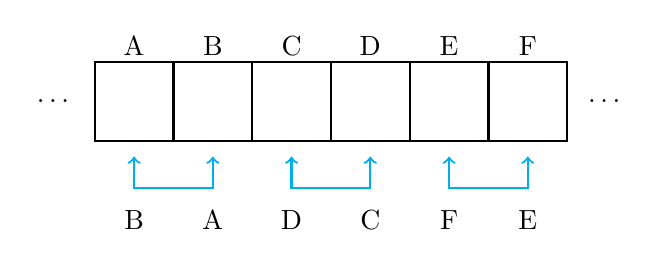
\begin{tikzpicture}
					% Parameters
					\def\boxwidth{1} % Width of each box
					\def\numboxes{6} % Total number of boxes
					\pgfmathtruncatemacro{\lastindex}{\numboxes-2} % Compute the last valid index for swapping
					\pgfmathtruncatemacro{\lastindexLet}{\numboxes-1} % Compute the last valid index for swapping


					% Draw the rectangle (sequence of letters)
					\draw[thick] (0, 0) rectangle (\numboxes*\boxwidth, 1);
					\foreach \i in {1,...,\numboxes} {
							\draw[thick] (\i*\boxwidth, 0) -- (\i*\boxwidth, 1);
						}

					% Add ellipses on both sides
					\node at (-0.5, 0.5) {\dots};
					\node at (\numboxes*\boxwidth+0.5, 0.5) {\dots};

					% Add arrows for swapping
					\foreach \i in {0,2,...,\lastindex} {
							\pgfmathsetmacro{\xstart}{\i*\boxwidth + 0.5*\boxwidth}
							\pgfmathsetmacro{\xend}{\xstart + \boxwidth}
							\draw[thick, cyan, <->] (\xstart, -0.2) -- (\xstart, -0.6) -- (\xend, -0.6) -- (\xend, -0.2);
						}

					% Add letters above the boxes
					\foreach \i in {0,...,\lastindexLet} {
							\pgfmathsetmacro{\xpos}{\i*\boxwidth + 0.5*\boxwidth}
							\pgfmathtruncatemacro{\letter}{65+\i} % ASCII value of A is 65
							\node at (\xpos, 1.2) {\char\letter};
						}

					% Add swapped letters below the boxes
					\foreach \i in {0,...,\lastindexLet} {
							\pgfmathsetmacro{\xpos}{\i*\boxwidth + 0.5*\boxwidth}
							\ifodd\i
								\pgfmathtruncatemacro{\swapletter}{65+\i-1} % ASCII value of A is 65
							\else
								\pgfmathtruncatemacro{\swapletter}{65+\i+1} % ASCII value of A is 65
							\fi
							\node at (\xpos, -1) {\char\swapletter};
						}
				\end{tikzpicture}
				\caption{\enquote{Zweiertausch}}
			\end{subfigure}
			\hfill
			\begin{subfigure}[b]{0.45\textwidth}
				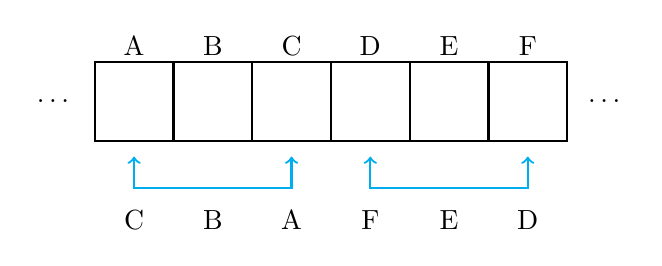
\begin{tikzpicture}
					% Parameters
					\def\boxwidth{1} % Width of each box
					\def\numboxes{6} % Total number of boxes
					\pgfmathtruncatemacro{\lastindex}{\numboxes-3} % Compute the last valid index for swapping
					\pgfmathtruncatemacro{\lastindexLet}{\numboxes-1} % Compute the last valid index for swapping


					% Draw the rectangle (sequence of letters)
					\draw[thick] (0, 0) rectangle (\numboxes*\boxwidth, 1);
					\foreach \i in {1,...,\numboxes} {
							\draw[thick] (\i*\boxwidth, 0) -- (\i*\boxwidth, 1);
						}

					% Add ellipses on both sides
					\node at (-0.5, 0.5) {\dots};
					\node at (\numboxes*\boxwidth+0.5, 0.5) {\dots};

					% Add arrows for swapping
					\foreach \i in {0,3,...,\lastindex} {
							\pgfmathsetmacro{\xstart}{\i*\boxwidth + 0.5*\boxwidth}
							\pgfmathsetmacro{\xend}{\xstart + \boxwidth*2}
							\draw[thick, cyan, <->] (\xstart, -0.2) -- (\xstart, -0.6) -- (\xend, -0.6) -- (\xend, -0.2);
						}

					% Add letters above the boxes
					\foreach \i in {0,...,\lastindexLet} {
							\pgfmathsetmacro{\xpos}{\i*\boxwidth + 0.5*\boxwidth}
							\pgfmathtruncatemacro{\letter}{65+\i} % ASCII value of A is 65
							\node at (\xpos, 1.2) {\char\letter};
						}

					% Add swapped letters below the boxes
					\foreach \i in {0,3,...,\lastindex} {
							\pgfmathtruncatemacro{\swapletter}{65+\i+2} % ASCII value of A is 65
							\pgfmathsetmacro{\xpos}{\i*\boxwidth + 0.5*\boxwidth}
							\node at (\xpos, -1) {\char\swapletter};
						}

					\foreach \i in {2,5,...,\numboxes} {
							\pgfmathtruncatemacro{\swapletter}{65+\i-2} % ASCII value of A is 65
							\pgfmathsetmacro{\xpos}{\i*\boxwidth + 0.5*\boxwidth}
							\node at (\xpos, -1) {\char\swapletter};
						}

					\foreach \i in {1,4,...,\lastindexLet} {
							\pgfmathtruncatemacro{\swapletter}{65+\i} % ASCII value of A is 65
							\pgfmathsetmacro{\xpos}{\i*\boxwidth + 0.5*\boxwidth}
							\node at (\xpos, -1) {\char\swapletter};
						}
				\end{tikzpicture}
				\caption{\enquote{Dreiertausch}}
			\end{subfigure}
			\caption{\enquote{Zweiertausch} und \enquote{Dreiertausch}}
			\label{fig:transposition-cipher}
		\end{figure}
	\end{myanswer}
\end{myexercise}


\subsection{Skytale}
Das Kyrptosystem \textit{Skytale} wurde bereits von den Griechen für militärische Zwecke verwendet. Der Verschlüsselungsalgorithmus kann wie folgt beschrieben werden:
\begin{itemize}
	\item Schreibe den Klartext zeilenweise in eine Tabelle (Matrix) von links nach rechts.
	\item Allfällige leere Felder in der letzten Zeile der Tabelle werden mit beliebigen Buchstaben gefüllt.
	\item Den Kryptotext erhalten wir, indem wir die Buchstaben Spalte für Spalte von links nach rechts und von oben nach unten lesen.
\end{itemize}

Praktisch umgesetzt werden kann dieser Algorithmus mit einem Stab und einem Band, siehe \cref{fig:skytale-band}. Die Anzahl Zeichen, die auf eine Windung des Bandes um den Stab passen, entspricht der Anzahl Zeilen in der Tabelle. Diese Anzahl, also die Anzahl Zeilen, entspricht dem Schlüssel des Skytale-Verschlüsselungsverfahrens.

\begin{figure}[H]
	\centering
	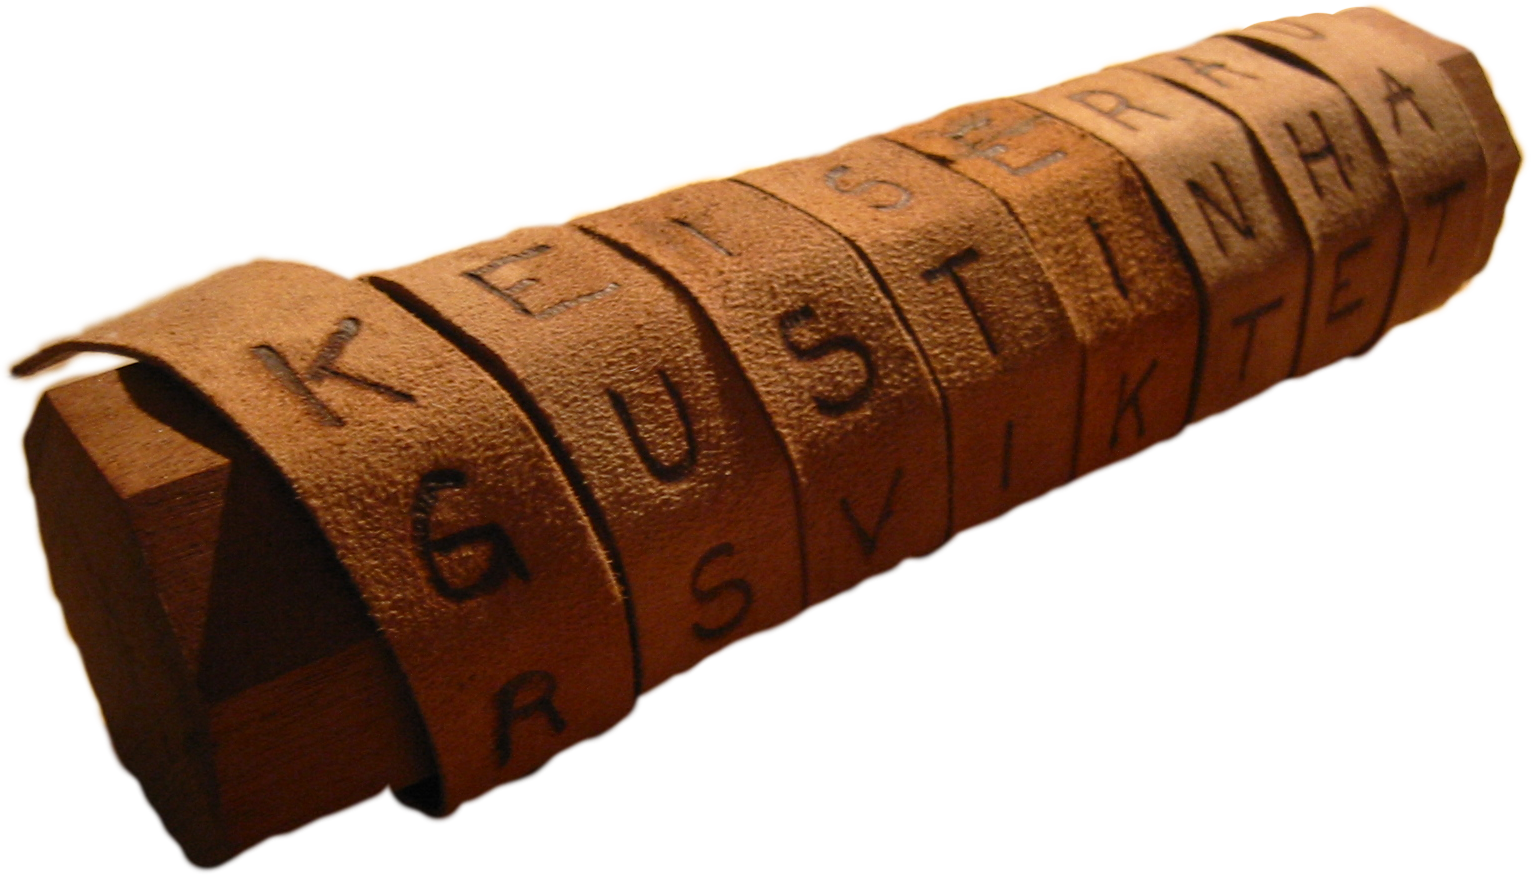
\includegraphics[width=0.5\linewidth]{Grundlagen_Info/03_Kryptologie/Figures/SkytaleWiki}
	\caption{Praktische Umsetzung der Skytale-Verschlüsselung mit einem Stab und einem Band \href{https://commons.wikimedia.org/wiki/File:Skytale.png}{Quelle}}
	\label{fig:skytale-band}
\end{figure}

\begin{myexercise}
	Der Kryptotext
	\begin{center}
		WNGIAEIEMATSMKRTTEAGIEINANINTUGNDOJEEENL
	\end{center}
	wurde mit einer Tabelle mit 5 Zeilen und 8 Spalten erzeugt. Wie lautet der Klartext?
	\begin{myanswer}

		Wir beginnen mit einer leeren $5\times 8$ Tabelle und schreiben den Kryptotext spaltenweise (von rechts nach links und von oben nach unten) in die leere Tabelle. Damit erhalten wir:
		\begin{table}[H]
			\centering
			\begin{tabular}{c|c|c|c|c|c|c|c}
				W & E & T & T & I & N & G       & E       \\ \hline
				N & I & S & T & E & I & N       & E       \\ \hline
				G & E & M & E & I & N & D       & E       \\ \hline
				I & M & K & A & N & T & O       & N       \\ \hline
				A & A & R & G & A & U & \red{J} & \red{L} \\
			\end{tabular}
		\end{table}
		Der Klartext
		\begin{center}
			Wettingen ist eine Gemeinde im Kanton Aargau
		\end{center}
		lässt sich nun einfach ablesen.
	\end{myanswer}
\end{myexercise}

\begin{myexercise}
	Der folgende Kryptotext der Länge 75 wurde mit SKYTALE verschlüsselt:
	\begin{center}
		ETIFIITNUTNFGENKURRELEODIERSILIMSEANIE\\
		MRECREMRHSNSSAPSTCBRCRHEUHORRNHNIEGEG
	\end{center}
	Dabei konnten mit dem Klartext \textbf{alle Zeilen der Tabelle vollständig aufgefüllt} werden.
	\begin{enumerate}
		\item Welches ist hier der Schlüssel, d.h. die Anzahl Zeichen auf einer Windung (bzw. Anzahl Zeilen der Tabelle)? Tipp: Probieren Sie die Schlüssel 3 und 5 aus. Sie können \href{https://cryptbreaker.marcwidmer.xyz/solve}{diesen Link}, Entschlüsselungswerkzeug \enquote{Tabelle} dazu verwenden.
		\item Wie lautet der Klartext?
		\item Wie viele Schlüssel müssen im schlimmsten Fall ausprobiert werden, bis der korrekte Schlüssel gefunden wurde? Das heisst, wie viele potentielle Schlüssel gibt es? Es gilt immer noch, dass alle Zeilen der Tabelle vollständig befüllt waren.
	\end{enumerate}

	\begin{myanswer}
		\begin{table}[H]
			\centering
			\begin{tabular}{c|c|c|c|c|c|c|c|c|c|c|c|c|c|c}
				E & I & N & K & L & E & I & N & E & R & S & C & H & R & I \\ \hline
				T & T & F & U & E & R & M & I & C & H & A & B & E & R & E \\ \hline
				I & N & G & R & O & S & S & E & R & S & P & R & U & N & G \\ \hline
				F & U & E & R & D & I & E & M & E & N & S & C & H & H & E \\ \hline
				I & T & N & E & I & L & A & R & M & S & T & R & O & N & G \\
			\end{tabular}
		\end{table}
		\begin{enumerate}
			\item Durch Ausprobieren finden wir, dass die Wahl des Schlüssels 5 zu einem sinnvollen Klartext führt, die Wahl des Schlüssels 3 jedoch nicht.

			\item
			      Der Klartext lautet also:
			      \begin{center}
				      {\small
					      EIN KLEINER SCHRITT FUER MICH ABER EIN GROSSER\\
					      SPRUNG FUER DIE MENSCHHEIT NEIL ARMSTRONG}
			      \end{center}
			\item Wir müssen $75=3\cdot 5\cdot 5$ Buchstaben auf ein Rechteck verteilen. Damit könnten $3, 5, 15$ und $25$ mögliche Schlüssel sein. $1$ und $75$ sind keine Schlüssel, da der gegebene Text kein Klartext ist.
		\end{enumerate}
	\end{myanswer}


\end{myexercise}
\begin{mychallenge}
	Sie möchten einen Klartext der Länge 87 mit Hilfe einer Tabelle mit 10 Zeilen chiffrieren. Wie viele Spalten benötigt diese Tabelle?

	\begin{myanswer}
		Die Tabelle benötigt 9 Spalten. Allgemein lässt sich die Anzahl benötigter Spalten berechnen durch
		\begin{align*}
			\ceil{\frac{\text{Länge des Textes}}{\text{Anzahl Zeilen}}}\quad(\text{``}\ceil{...}\text{'' bedeutet ``nach oben aufgerundet'')}.
		\end{align*}
	\end{myanswer}
\end{mychallenge}

\subsection{Caesar}
\label{subsec:caesar}
Eines der bekanntesten Verschlüsselungssysteme der Antike ist die Caesar-Verschlüsselung, die von Julius Caesar verwendet wurde. Dieses Verschlüsselungssystem besteht essentiell aus einer Verschiebung aller Buchstaben um eine vordefinierte Anzahl Positionen im Alphabet. Der \tib{Schlüssel} bezeichnet dabei die Anzahl Positionen, um die jeder Buchstabe verschoben wird. Ausgedrückt wird der Schlüssel auch als Buchstabe, der dem Buchstaben A entsprechen würde.

\begin{myexample}
Mit dem Schlüssel ``D'' (3 Positionen) würde das Wort ``HALLO'' als ``KDOOR'' geschrieben:
\begin{figure}[H]
	\centering
	\caesar[3]
\end{figure}
\end{myexample}

Der Schlüssel ``B'' bedeutet also eine Verschiebung um 1 Position, ``C'' um 2 Positionen, ``D'' um drei Positionen usw. Im Allgemeinen lässt sich die Verschiebung folgendermassen schreiben:

$\text{Verschiebung = Ord}(\square)$, wobei $\text{Ord}(A)=0$.

\begin{myexample}
Folgender Text wurde mit dem Schlüssel ``G'' (6 Positionen) verschlüsselt:

\begin{verbatim}
  Klartext: JEMANDMUSSTEJOSEFKVERLEUMDETHA...
 Schlüssel: GGGGGGGGGGGGGGGGGGGGGGGGGGGGGG...
Kryptotext: PKSGTJSAYYZKPUYKLQBKXRKASJKZNG...
\end{verbatim}

\end{myexample}

\begin{myexercise}
	Der Kryptotext
	\begin{center}
		\texttt{X G T Y G P F G U E J N W G U U G N B Y G K}
	\end{center}
	wurde mit CAESAR verschlüsselt, der Schlüssel ist aber unbekannt.
	Entschlüsseln Sie den Kryptotext, ohne alle Schlüssel auszuprobieren, wenn Sie wissen, dass der häufigste Buchstabe im Klartext \texttt{E} ist.
	\begin{myanswer}
		Der häufigste Buchstabe im Kryptotext ist ``G'' Wir können den Text mithilfe der folgenden Verschiebung entschlüsseln (G $\rightarrow$ E) :
		\begin{center}
			\caesar[2]\\
			\texttt{V E R W E N D E D E N S C H L U E S S E L Z W E I}
		\end{center}
	\end{myanswer}
\end{myexercise}


% \begin{mychallenge}
% Implementieren Sie die Caesar-Verschlüsselung in Python. Einige nützliche Funktionen, die Sie für Zeichenketten verwenden können, finden SIe in:
%
%
% \begin{myanswer}
% \lstinputlisting{Grundlagen_Info/03_Kryptologie/Python package/encryption/caesar.py}
% \end{myanswer}
% \end{mychallenge}

\subsubsection{Knacken von Caesar}
\begin{itemize}
	\item Einerseits reicht es, alle 25 möglichen Verschiebungen auszuprobieren. Ein moderner Computer hat dies in einigen Milisekunden erledigt.
	\item Andererseits kann, wenn der Text genügend lange ist, anhand der Häufigkeit der verschlüsselten Buchstaben mittels Häufigeitsanalyse in kürzester Zeit bestimmt werden, was der Schlüssel war. \cref{fig:caesar-freq} zeigt die Häufigkeiten der Buchstaben eines langen, mit Caesar verschlüsselten Texts im Kryptotext.
\end{itemize}

\begin{figure}[H]
	\centering
	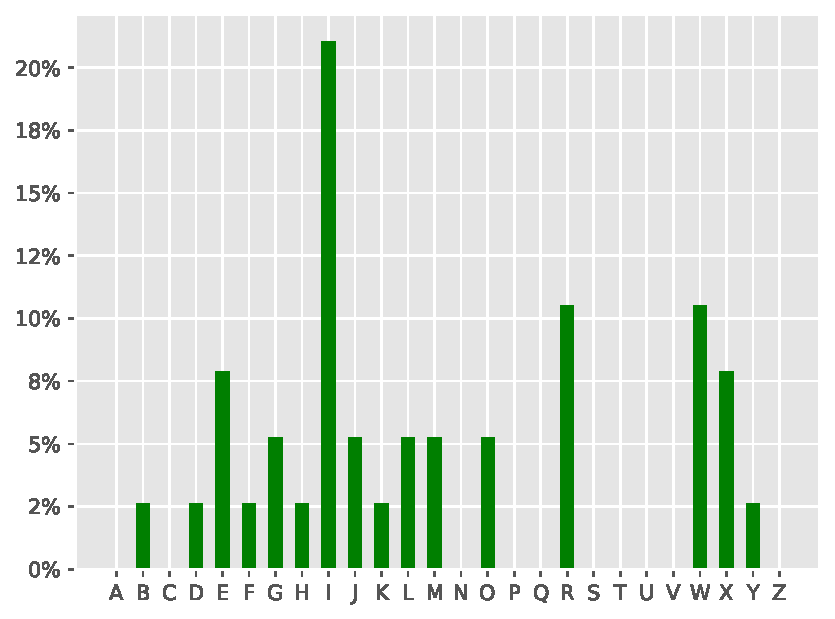
\includegraphics[width=0.7\linewidth]{Grundlagen_Info/03_Kryptologie/Figures/caesar-freq-exercise}
	\caption{Buchstabenhäufigkeit in einem nach Caesar verschlüsselten Text}
	\label{fig:caesar-freq}
\end{figure}

Die durchschnittlichen Häufigkeiten von Buchstaben, Bi- und Tri-Grammen in deutschen Texten ist in \cref{tab:alle-haeufigkeiten} angegeben.

\begin{table}[H]
	\centering
	\begin{subtable}[t]{0.3\textwidth}
		\centering
		\begin{tabular}{c|p{1.9cm}}
			\textbf{Buchstabe} & Relative Häufigkeit (\%) \\ \midrule
			E                  & 17.40                    \\ \midrule
			N                  & 9.78                     \\ \midrule
			I                  & 7.55                     \\ \midrule
			S                  & 7.27                     \\ \midrule
			R                  & 7.00                     \\ \midrule
			A                  & 6.51                     \\ \midrule
			T                  & 6.15                     \\ \midrule
			D                  & 5.08                     \\ \midrule
			H                  & 4.76                     \\ \midrule
			U                  & 4.35                     \\
		\end{tabular}
		\caption{Buchstabenhäufigkeit}
	\end{subtable}
	\hspace{0.5cm}
	\begin{subtable}[t]{0.3\textwidth}
		\centering
		\begin{tabular}{c|p{1.9cm}}
			\textbf{Bigramm} & Relative Häufigkeit (\%) \\ \midrule
			ER               & 3.94                     \\ \midrule
			EN               & 3.07                     \\ \midrule
			CH               & 2.73                     \\ \midrule
			DE               & 2.41                     \\ \midrule
			EI               & 2.29                     \\ \midrule
			ND               & 2.07                     \\ \midrule
			IE               & 1.97                     \\ \midrule
			GE               & 1.88                     \\ \midrule
			TE               & 1.88                     \\ \midrule
			IN               & 1.82                     \\
		\end{tabular}
		\caption{Bigrammhäufigkeit}
	\end{subtable}
	\hspace{0.5cm}
	\begin{subtable}[t]{0.3\textwidth}
		\centering
		\begin{tabular}{c|p{1.9cm}}
			\textbf{Trigramm} & Relative Häufigkeit (\%) \\ \midrule
			DER               & 1.44                     \\ \midrule
			SCH               & 1.21                     \\ \midrule
			ICH               & 1.08                     \\ \midrule
			DIE               & 0.98                     \\ \midrule
			UND               & 0.95                     \\ \midrule
			DEN               & 0.78                     \\ \midrule
			CHE               & 0.77                     \\ \midrule
			EIN               & 0.75                     \\ \midrule
			NDE               & 0.74                     \\ \midrule
			GEN               & 0.72                     \\
		\end{tabular}
		\caption{Trigrammhäufigkeit}
	\end{subtable}
	\caption{Relative Häufigkeiten der Buchstaben, Bigramme und Trigramme im Deutschen}
	\label{tab:alle-haeufigkeiten}
\end{table}



\begin{myexercise}\label{ex:caesar}
	Können Sie aus \cref{tab:alle-haeufigkeiten} entschlüsseln, was der Klartext ist?

	Kryptotext:

	\texttt{WMILEFIRIWKIWGLEJJXHMIWIRXIBXDYOREGOIR}

	\begin{myanswer}
		Offensichtlich ist der häufigste Buchstabe im Kryptotext ``I'' und der häufigste Buchstabe in deutschen Texten ist der Buchstabe ``E'', wir haben hier also vermutlich eine Verschiebung von ``E'' zu ``I'', also eine Verschiebung um 4 Stellen. Der Klartext lautet daher: \texttt{SIEHABENESGESCHAFFTDIESENTEXTZUKNACKEN}
	\end{myanswer}
\end{myexercise}

\begin{mychallenge}
	Kann man immer wie in \cref{ex:caesar} vorgehen? In welchen Fällen funktioniert dieses Vorgehen eventuell nicht?
	\begin{myanswer}
		Falls der Text zu kurz ist, funktioniert die Häufigkeitsanalyse nicht immer, da der häufigste Buchstabe im Originaltext nicht immer der Buchstabe ``E'' ist. Dies wird beispielsweise im Wort ``Wort'' illustriert, das keinen Buchstaben ``E'' enthält. In diesem Fall müsste man alle 26 möglichen Verschiebungen durchprobieren.
	\end{myanswer}
\end{mychallenge}

\begin{mychallenge}
	Um zu verschlüsseln, liest man die Caesar-Scheibe von innen (Klartext) nach aussen (Kryptotext). Um zu entschlüsseln, liest man von aussen (Kryptotext) nach innen (Klartext). Gibt es Schlüssel bei Caesar, bei denen es sowohl für die Ver- wie Entschlüsselung keine Rolle spielt, in welche Richtung man die Scheiben liest?
	\begin{myanswer}
		Ja, dies tritt bei Schlüsseln 0 (A, keine Verschlüsselung) und 13 (N, die Hälfte des Alphabets) auf.
	\end{myanswer}
\end{mychallenge}

\subsection{Monoalphabetische Substitution}

Eine Weiterentwicklung der Caesar-Veschlüsselung besteht darin, nicht jeden Buchstaben im Klartext um dieselbe Anzahl Positionen zu verschieben, sondern für jeden Klartext-Buchstaben $B_K$ einen Kryptotext-Buchstaben $B_G$ zu definieren, durch den der Buchstabe ersetzt wird (siehe \cref{fig:monoalph-subst}).

\begin{figure}[H]
	\centering
	\multiKey{Z,E,A,B,C,D,Y,X,W,H,I,V,U,T,G,F,J,K,R,Q,L,M,S,N,P,O}
	\caption{Monoalphabetische Substitution}
	\label{fig:monoalph-subst}
\end{figure}

Diese Verschlüsselungsmethode kann nicht geknackt werden, indem alle Buchstaben um gleich viele Positionen verschoben werden. Man kann also nicht lediglich alle 25 möglichen Verschiebungen ausprobieren.

Obschon es nun eine Vielzahl möglicher Schlüssel gibt, kann diese Verschlüsselungsmethode ebenfalls sehr einfach geknackt werden per Häufigkeitsanalyse, die wir bereits in \cref{subsec:caesar} gesehen und in \cref{ex:caesar} mittels \cref{tab:alle-haeufigkeiten} durchgeführt haben.

\begin{myexample}
Folgender Kryptotext wurde abgefangen:

\texttt{MUMMUXJUQYMHQOUSUTUQNGWTJQVHUMXQUXQJSUVYPPUM}

Wir wissen, dass er per monoalphabetische Verschlüsselung erstellt wurde, wie beispielsweise in \cref{fig:monoalph-subst}, kennen jedoch den Schlüssel nicht. Wir verwenden \cref{tab:alle-haeufigkeiten}, um den Schlüssel zu erraten und den Text zu entschlüsseln. Dabei gehen wir wie folgt vor:

\begin{itemize}
	\item Wir beginnen damit, die häufigsten Buchstaben zu zählen: U kommt 10-mal vor, M kommt 6-mal vor, Q kommt 6-mal vor. Aufgrund von \cref{tab:alle-haeufigkeiten} versuchen wir, folgendes einzusetzen: \texttt{U=E, M=N, Q=I}. Wir erhalten folgenden Teil-Klartext:
	      \begin{verbatim}
KRYPTOTEXT: MUMMUXJUQYMHQOUSUTUQNGWTJQVHUMXQUXQJSUVYPPUM
KLARTEXT:   NENNE--EI-N-I-E-E-EI-----I--EN-IE-I--E----EN
    \end{verbatim}
	\item Nun könnten wir weiterfahren, indem wir die häufigsten Trigramme anschauen. Dabei suchen wir im bisherigen Klartext nach Klartext-Teilen, wo wir Trigramme einsetzen könnten. Laut \cref{tab:alle-haeufigkeiten} ist ein häufiges Trigramm in deutschen Texten \texttt{``DIE''}. Dieses probieren wir einzusetzen (D=X):

	      \begin{verbatim}
KRYPTOTEXT: MUMMUXJUQYMHQOUSUTUQNGWTJQVHUMXQUXQJSUVYPPUM
KLARTEXT:   NENNED-EI-N-I-E-E-EI-----I--ENDIEDI--E----EN
    \end{verbatim}
	\item Der Klartext nimmt langsam Form an und wir können nun damit beginnen, verbleibende Worte zu erraten. Könnte es sich beim ersten Wort um das Wort ``\texttt{DREI}'' handeln? Wir setzen ein:
	      \begin{verbatim}
KRYPTOTEXT: MUMMUXJUQYMHQOUSUTUQNGWTJQVHUMXQUXQJSUVYPPUM
KLARTEXT:   NENNEDREI-N-I-E-E-EI----RI--ENDIEDIR-E----EN
    \end{verbatim}
	\item Sobald einzelne Wörter erkannt werden, können wir sie mit Trennlinien voneinander abgrenzen:
	      \begin{verbatim}
KRYPTOTEXT: MUMMU|XJUQ|YMHQOUSUTUQNGWTJQVHUM|XQU|XQJ|SUVYPPUM
KLARTEXT:   NENNE|DREI|-N-I-E-E-EI----RI--EN|DIE|DIR|-E----EN
\end{verbatim}
	\item Wir fahren durch Ausprobieren und Erraten weiter, bis das Lösungswort gefunden ist:
	      \begin{verbatim}
KRYPTOTEXT: MUMMU|XJUQ|YMHQOU|SUTUQNGWTJQVHUM|XQU|XQJ|SUVYPPUM
KLARTEXT:   NENNE|DREI|ANTIKE|GEHEIMSCHRIFTEN|DIE|DIR|GEFALLEN
\end{verbatim}
\end{itemize}
Je länger ein Text ist, desto zuverlässiger funktioniert das Erraten der Buchstaben per Häufigkeitsanalyse.
\end{myexample}

\begin{myexercise}
	Entschlüsseln Sie den Text ``\texttt{ECRRCKZVRAZCRZK}'' mit dem Schlüssel aus \cref{fig:monoalph-subst}.
	\begin{myanswer}
		BESSERALSCAESAR
	\end{myanswer}
\end{myexercise}

\begin{mychallenge}
	Lösen Sie eine Knobelaufgabe aus dem Kapitel ``\href{https://cryptbreaker.marcwidmer.xyz/problems/substitution}{Substitution}''.
\end{mychallenge}


\begin{mychallenge}
	Wie viele Verschlüsselungs-Möglichkeiten gibt es in der Verschlüsselungsmethode aus \cref{fig:monoalph-subst}?
	\begin{myanswer}
		Für jeden Buchstaben gibt es 26 mögliche Verschiebungen (keine Verschiebung ist auch eine Möglichkeit), also gibt es insgesamt $26^{26}$ mögliche Verschiebungen.
	\end{myanswer}
\end{mychallenge}

\subsection{Vigenère}
% \iftoggle{teacherToggle}{
% 	\begin{myExBox}[Einführung]
% 		\tcbsubtitle{Thema}
% 		Das zweite Modul (Ganz-Klassenlektion und Programmier-Doppellektion) zeigt den SuS zuerst auf, dass alle monoalphabetischen Kryptosysteme mittels Häufigkeitsanalyse geknackt werden können. Die SuS werden danach in polyalphabetische Verschlüsselungsverfahren eingeführt. Schlussendlich wird aufgezeigt, dass auch diese mit Häufigkeitsanalyse geknackt werden können, solange die Schlüssellänge deutlich kürzer als die Klartextlänge ist..


% 		\tcbsubtitle{Operationalisierte Lernziele}
% 		\begin{todolist}
% 			\item Die SuS können mit einen beliebigen monoalphabetischen Text ausreichender Länge mittels Häufigkeitsanalyse knacken.
% 			\item Die SuS können einen Text mit Vigenère ver- und entschlüsseln.
% 			\item Die SuS können die Friedman'sche Charakteristik anwenden, um die Schlüssellänge eines mit Vigenère verschlüsselten Kryptotexts zu bestimmen
% 			\item Die SuS können einen Vigenère-Kryptotext, dessen Schlüssellänge bekannt ist, mittels Häufigkeitsanalyse entschlüsseln.
% 			\item Die SuS können einen Text mittels OTP verschlüsseln und wissen, weshalb diese Verschlüsselungsmethode als sicher gilt.
% 		\end{todolist}

% 		\tcbsubtitle{Grober Lektionsablauf}
% 		...
% 		\begin{myExBox}[title=Mögliche Schwierigkeiten \& geeignete Massnahmen]
% 			\begin{enumerate}
% 				\item ...
% 			\end{enumerate}
% 		\end{myExBox}
% 	\end{myExBox}
% 	\newpage\stepcounter{dlcounter}
% }{}
Wie wir in \cref{ex:caesar} gesehen haben, ist es extrem einfach, Text, die mit Caesar verschlüsselt worden sind, anzugreifen, entweder mittels Buchstabenhäufigkeitsanalyse oder indem man einfach alle 25 möglichen Verschiebungen ausprobiert. Auch weitere monoalphabetische Substitutions-Verfahren wie \cref{fig:monoalph-subst} können durch etwas Knobeln relativ einfach geknackt werden.

Vigenère hatte eine andere Idee: Statt den ganzen Text mit einem einzigen Schlüssel zu verschlüsseln, verwendete er ein Wort, mit welchem er den Text ``zyklisch'', also gruppenweise verschlüsselte.

\begin{myexample}\label{ex:vigenere}
Wenn der Schlüssel beispielsweise ``KEY'' war, wurden die Buchstaben folgendermassen verschlüsselt (siehe Beispiel unterhalb):
\begin{itemize}
	\item Buchstaben 1, 4, 7, 10 etc. mit ``K''
	\item Buchstaben 2, 5, 8, 11 etc. mit ``E''
	\item Buchstaben 3, 6, 9, 12 etc. mit ``Y''
\end{itemize}

\begin{figure}[H]
	\begin{verbatim}
  Klartext: JEM|AND|MUS|STE|JOS|EFK|VER|LE...
 Schlüssel: KEY|KEY|KEY|KEY|KEY|KEY|KEY|KE...
Kryptotext: TIK|KRB|WYQ|CXC|TSQ|OJI|FIP|VI...
\end{verbatim}
\end{figure}

Im Vergleich dazu wird bei Caesar jeder Buchstabe durch \textit{denselben} Schlüssel verschlüsselt, beispielsweise:
\begin{verbatim}
  Klartext: JEMANDMUSSTEJOSEFKVERLEUMDETHA...
 Schlüssel: GGGGGGGGGGGGGGGGGGGGGGGGGGGGGG...
Kryptotext: PKSGTJSAYYZKPUYKLQBKXRKASJKZNG...
\end{verbatim}
\end{myexample}

Wie Sie wissen, ist der Buchstabe ``E'' der häufigste Buchstabe in deutschen Texten. Diese Eigenschaft haben wir uns in \cref{ex:caesar} zunutze gemacht, um den Text zu knacken. Da bei Vigenère jedoch der Buchstaben nun nicht mehr immer mit demselben Schlüssel verschlüsselt ist, sondern je nach Position mit dem Schlüssel ``K'', ``E'', oder ``Y'', wird der Buchstabe ``E'' im Kryptotext nun breiter auf andere Buchstaben verteilt (siehe \cref{fig:ex-vigenere-e}). Anders gesagt, ein Buchstabe im Kryptotext repräsentiert nun nicht mehr immer den gleichen Buchstaben im Klartext, sondern kann einen von drei Buchstaben repräsentieren.

\begin{figure}[H]
	\centering
	\begin{subfigure}{.45\textwidth}
		\centering
		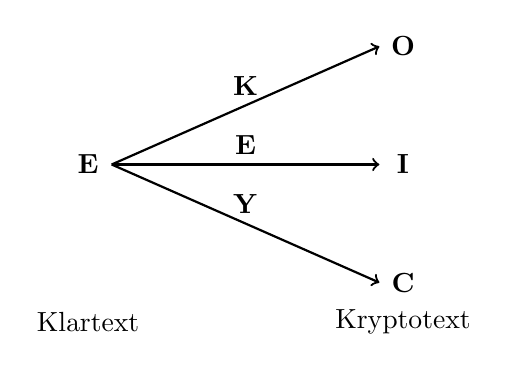
\begin{tikzpicture}
			% Klartext und Kryptotext Labels
			\node at (0, 0) {\textbf{E}};
			\node at (4, 1.5) {\textbf{O}};
			\node at (4, 0) {\textbf{I}};
			\node at (4, -1.5) {\textbf{C}};

			% Verbindungspfeile mit Schlüsseln
			\draw[->, thick] (0.3, 0) -- (3.7, 1.5) node[midway, above] {\textbf{K}};
			\draw[->, thick] (0.3, 0) -- (3.7, 0) node[midway, above] {\textbf{E}};
			\draw[->, thick] (0.3, 0) -- (3.7, -1.5) node[midway, above] {\textbf{Y}};

			% Labels Klartext und Kryptotext
			\node[align=center] at (0, -2) {Klartext};
			\node[align=center] at (4, -2) {Kryptotext};
		\end{tikzpicture}
	\end{subfigure}
	\begin{subfigure}{.45\textwidth}
		\centering
		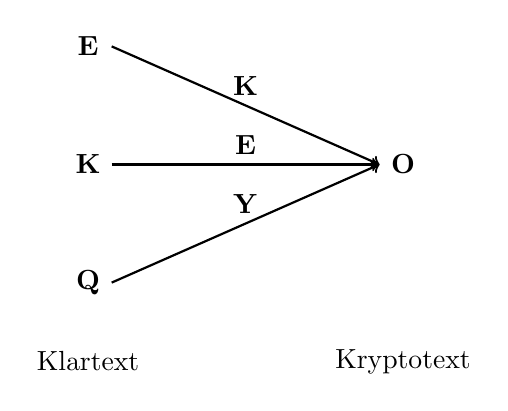
\begin{tikzpicture}
			% Klartext letters
			\node at (0, 1.5) {\textbf{E}};
			\node at (0, 0) {\textbf{K}};
			\node at (0, -1.5) {\textbf{Q}};

			% Kryptotext letter
			\node at (4, 0) {\textbf{O}};

			% Verbindungspfeile mit Schlüsseln
			\draw[->, thick] (0.3, 1.5) -- (3.7, 0) node[midway, above] {\textbf{K}};
			\draw[->, thick] (0.3, 0) -- (3.7, 0) node[midway, above] {\textbf{E}};
			\draw[->, thick] (0.3, -1.5) -- (3.7, 0) node[midway, above] {\textbf{Y}};

			% Labels Klartext und Kryptotext
			\node[align=center] at (0, -2.5) {Klartext};
			\node[align=center] at (4, -2.5) {Kryptotext};
		\end{tikzpicture}
	\end{subfigure}
	\caption{Verschlüsselungs-Möglichkeiten mit Vigenère, mit dem Schlüssel ``KEY'' aus \cref{ex:vigenere}}
	\label{fig:ex-vigenere-e}
\end{figure}

Diese Verschlüsslungsmethode galt während mehreren Jahrehunderten als sicher und war der Gold-Standard in vielen militärischen Verschlüsslungs-Anwendungen. Um einen Text zu verschlüsseln, wurde jeder Buchstabe im Klartext einzeln verschlüsselt, und je nach Schlüssel (z.B. ``K'', ``E'' oder ``Y'' in \cref{ex:vigenere}) wurde der entsprechende Buchstabe des Kryptotexts aus einer Tabelle herausgelesen (siehe \cref{tab:vigenere})


\cref{fig:langer-text-vig-caesar} zeigt die Buchstabenhäufigkeit im Kryptotext für einen langen Text, welcher einmal mit Caesar und einmal mit Vigenère verschlüsselt wurde.

\begin{figure}[H]
	\centering
	\begin{subfigure}{.49\linewidth}
		\centering
		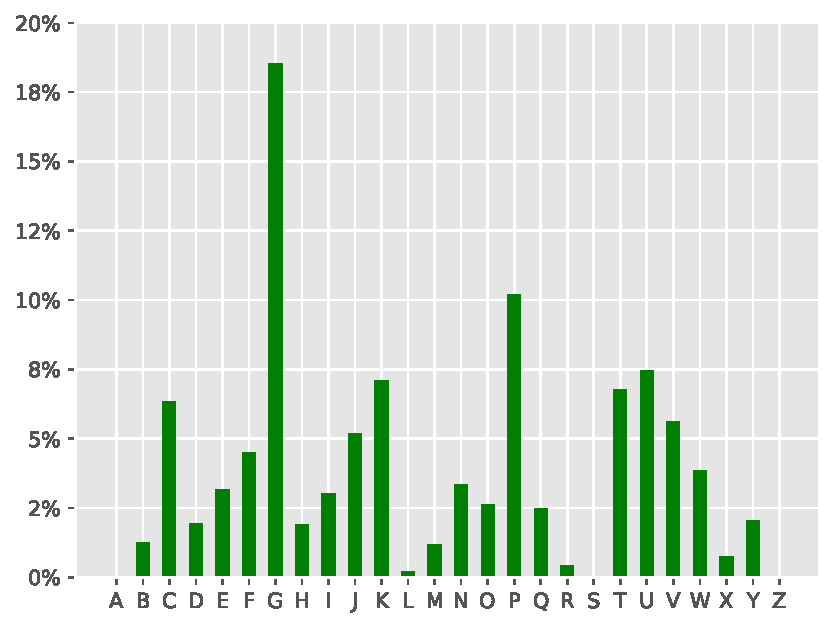
\includegraphics[width=\linewidth]{Grundlagen_Info/03_Kryptologie/Figures/caesar-freq}
		\caption{Caesar}
	\end{subfigure}
	\begin{subfigure}{.49\linewidth}
		\centering
		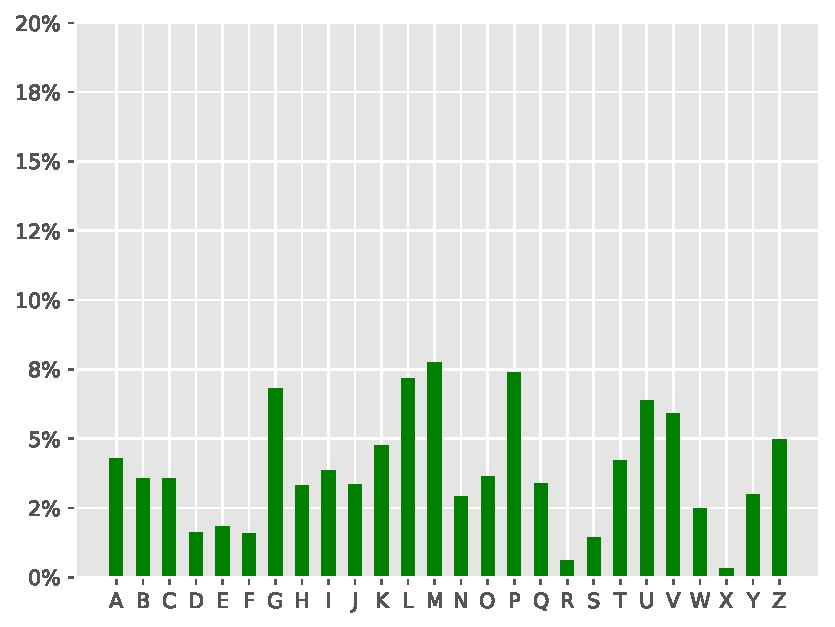
\includegraphics[width=\linewidth]{Grundlagen_Info/03_Kryptologie/Figures/vigenere-freq}
		\caption{Vigenère}

	\end{subfigure}
	\caption{Buchstabenhäufigkeit in einem langen Text, welcher mit unterschiedlichen Verfahren verschlüsselt wurde}
	\label{fig:langer-text-vig-caesar}
\end{figure}

\cref{fig:langer-text-vig-caesar} zeigt, dass Vigenère zu einer insgesamt homogeneren Verteilung aller Buchstaben im Kryptotext führt. Dies kommt daher, dass bei Vigenère jeder Klartext-Buchstaben auf \textit{mehrere} Kryptotext-Buchstaben verteilt wird, währenddem bei Caesar jeder Klartext-Buchstaben durch genau \textit{einen} Buchstaben im Kryptotext kodiert wird. \cref{tab:vigenere} zeigt die Vigenère-Tabelle, mithilfe welcher man einen Text mit der Vigenère-Methode ver- sowie entschlüsseln kann, sofern der Schlüssel bekannt ist. Folgende zwei Beispiele zeigen auf, wie diese Tabelle genutzt werden kann:

\begin{enumerate}
	\item \textbf{Verschlüsselung}: Soll beispielsweise der Klartext-Buchstabe \enquote{E} mit dem Schlüsselteil \enquote{K} verschlüsselt werden, so findet man in der Tabelle den entsprechenden Kryptotext-Buchstaben \enquote{O}.
	\item \textbf{Entschlüsselung}: Soll beispielsweise der Kryptotext-Buchstabe \enquote{O} mit dem Schlüsselteil \enquote{K} entschlüsselt werden, so sucht man in der Tabelle nach dem Klartext-Buchstaben, der mit \enquote{O} und \enquote{K} korrespondiert. Dies ist in diesem Fall der Buchstabe \enquote{E}.
\end{enumerate}

\begin{table}[H]
	\centering
	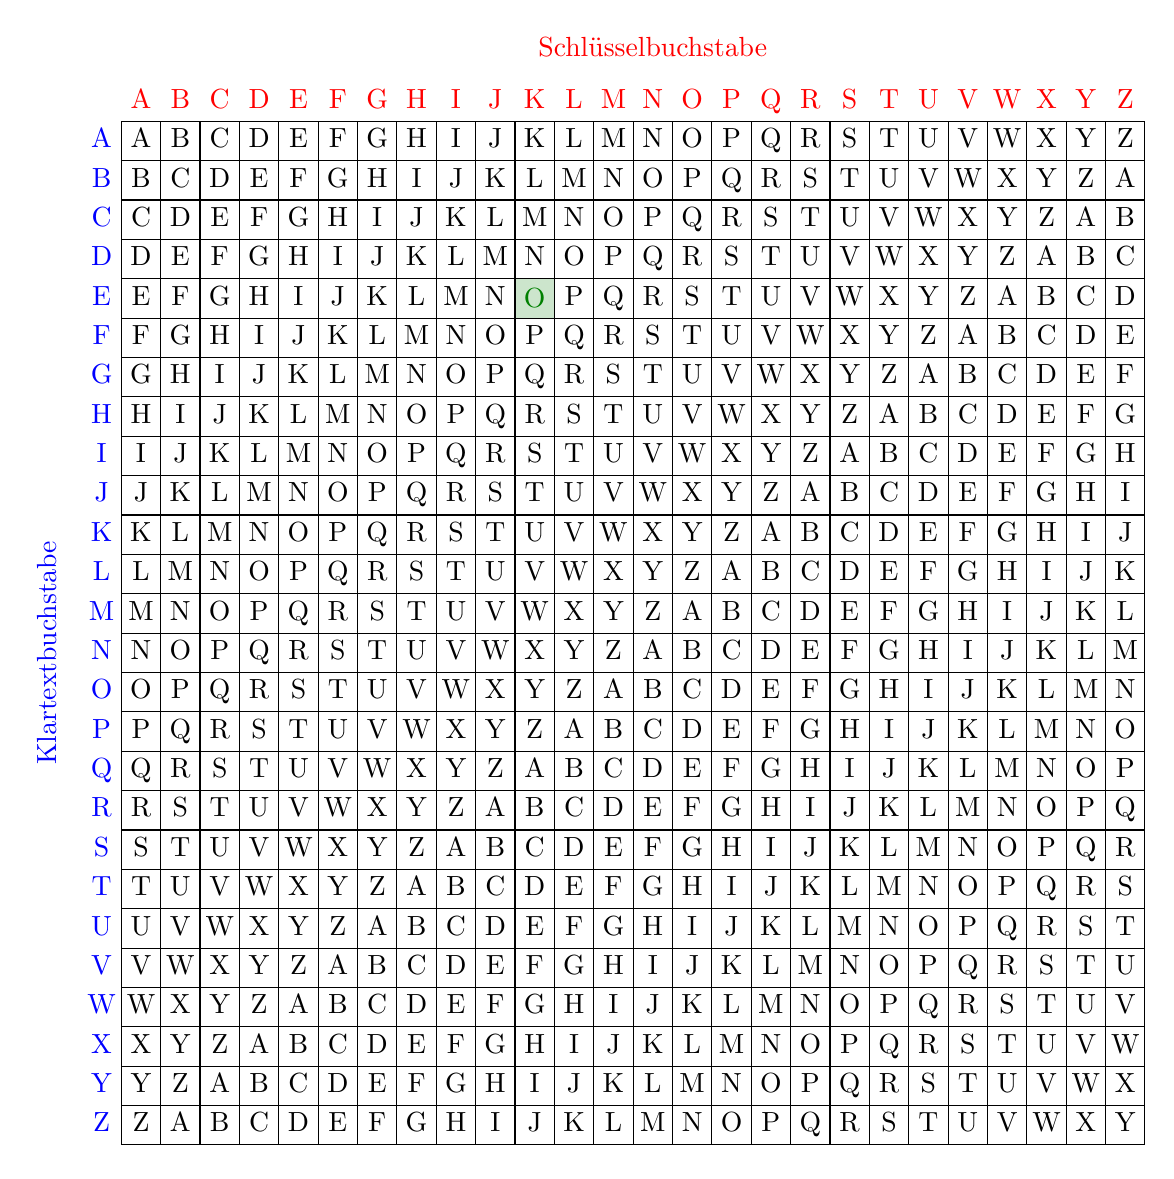
\begin{tikzpicture}
		\foreach \i in {0,...,25} {
				\node at (-0.5,-\i*0.5) {\textcolor{Blue}{\strut\symbol{\numexpr`A+\i\relax}}};
				\node at (\i*0.5,0.5) {\textcolor{Red}{\strut\symbol{\numexpr`A+\i\relax}}};
				\foreach \j in {0,...,25} {
						\edef\k{\ifnum\numexpr\i+\j\relax>25
								\the\numexpr\i+\j-26\relax
							\else
								\the\numexpr\i+\j\relax
							\fi}
						\node[draw,minimum size=0.5cm,inner sep=0pt]
						at (\i*0.5,-\j*0.5) {\strut\symbol{\numexpr`A+\k\relax}};
					}
			}
		\node[draw,minimum size=0.5cm,inner sep=0pt,fill=Green!20] at (5.0,-2.0) {\textcolor{Green}{O}};
		\node at (6.5,1.2) {\textcolor{Red}{Schlüsselbuchstabe}};
		\node[rotate = 90] at (-1.2,-6.5)  {\textcolor{Blue}{Klartextbuchstabe}};
	\end{tikzpicture}
	\caption{Vigenère-Tabelle}
	\label{tab:vigenere}
\end{table}


\begin{myexercise}
	\textbf{Entschlüsseln} Sie folgenden Text von Hand, wenn Sie wissen, dass er mit dem Schlüssel \enquote{\textcolor{red}{\texttt{TOP}}} und mit der Methode von Vigenère verschlüsselt worden ist:

	\texttt{UFPOCVNHVXAPVVI}
	\begin{myanswer}
		\textcolor{blue}{\texttt{BRAVOGUTGEMACHT}}
	\end{myanswer}
\end{myexercise}

\begin{myexercise}
	\textbf{Verschlüsseln} Sie folgenden Text von Hand, mit dem Schlüssel \enquote{\textcolor{red}{\texttt{YES}}} und mit der Methode von Vigenère:

	\textcolor{blue}{\texttt{NIEMANDKANNDASLESEN}}
	\begin{myanswer}
		\texttt{LMWKEFBOSLRVYWDCWWL}
	\end{myanswer}
\end{myexercise}

\subsubsection{Knacken von Vigenère}\label{subsubsec:vigHack}

Wenn die Schlüssellänge eines mit Vigenère verschlüsselten Texts bekannt ist, ist dieser relative einfach zu knacken: Man unterteilt den Text in diesem Fall einfach in Gruppen und geht für jede Gruppe gleich vor wie bei Caesar, um den Schlüssel zu finden.

\begin{myexample}
Angenommen, wir wüssten, dass folgender Text mit einem Schlüssel verschlüsselt worden ist, der drei Zeichen lang ist:

\texttt{\colorstring[ForestGreen,RoyalBlue,Crimson]{MKUMYBVFLZDHZGOMKAMTRMKAPCAUGPVGNIPGMULMNLMKUOGUWOTMPNTGPKJKMPZCGZAGUNTBMJSQPNAOVZILVFPMKJPOPBIHVBLUJLZBLVILVKLAULQEOJKUINSMKUCPKNTLCGTQEOUGPVGZTGIMPZQPKQGZMTNMILVFKQGMCGYAQSKJLAGLTGUOGZKJHNHLVKZBYPMFPMOLQPLQEOJKUAQNTWLKMSQEOUGPVDLAVLZUVOCUHKULGTOGMCGOTGCWPYCJPOGTLCZMKUDGYAWUSGULCZAOLQPLSWUAVKITBVVLZNLQFLBKJPMVMPUBGQMVGBPPKJAHGPKJUMPUQEOBGPVGUAVYQEOCPKJKUVKLMKUOTVMUZMTLZOHTGYOGDMULVCSAKULKLAGUIWNMPITKJSGUEGUVFHANPMDL}}


Den Schlüssel selbst kennen wir nicht, wir wissen jedoch, dass jeder der grün markierten Buchstaben beispielsweise mit demselben Buchstaben verschlüsselt worden ist. Wir können also für jede der Gruppen (grün, blau, rot) die Häufigkeit der Buchstaben betrachten (siehe \cref{fig:vig-subgroup}).

\begin{figure}[H]
	\centering
	\foreach \x in {1,...,3}{
			\begin{subfigure}{.3\linewidth}
				\centering
				\includegraphics[width=\linewidth]{Grundlagen_Info/03_Kryptologie/Figures/vigenere-len3-group\x}
				\caption{Untergruppe \x}
			\end{subfigure}
		}
	\caption{Buchstabenhäufigkeit in einem mit Vigenère verschlüsselten Text, pro Untergruppe}
	\label{fig:vig-subgroup}
\end{figure}

Dabei erkennen wir, dass die häufigsten Buchstaben pro Gruppe \textcolor{ForestGreen}{M}, \textcolor{RoyalBlue}{G}, bzw. \textcolor{Crimson}{L} sind. Wir haben es also mit folgenden Verschiebungen zu tun:
\begin{figure}[H]
	\centering
	\resizebox{.65\textwidth}{!}{\caesar[8] \caesar[2] \caesar[7]}
\end{figure}
Der Schlüssel muss demnach ``ICH'' sein und wir können den Text somit entschlüsseln.
\end{myexample}

\begin{myexercise}

	Kopieren Sie den folgenden Kryptotext und versuchen Sie, ihn mit dem \href{https://cryptbreaker.marcwidmer.xyz/solve}{Analysetool} zu entziffern, wenn Sie wissen, dass die Schlüssellänge drei ist. Schauen Sie sich die Buchstabenhäufigkeiten für jede der 3 Gruppen an, indem Sie unter \enquote{Analysewerkzeug} die Häufigkeitsanalyse auswählen und \textit{stride} (Schrittgrösse) 3. Unterhalb der Grafiken kann man zwischen jeder der drei Gruppen hin- und herwechseln. Probieren Sie den wahrscheinlichsten Schlüssel aus, indem Sie beim \enquote{Entschlüsselungswerkzeug} \enquote{Vigenère} auswählen und den Schlüssel eingeben.

	\texttt{\colorstring[black]{WORBHHHLUQOWWLDSYSQOWOUKSUDSNEGAAZAEBKISMRILHGPCVLIBZTRLMHYUSIEBILWJKULZSPGHCEFZUQOIQOWCOLSBCVKISZMOSFSZTNBHOSTSUFILHZPCVTEWUHSYZBVCVQEBLMKHHBNEBLIUAIVYDFHEBNTSBCVGUBBNUBTGVMCLGHPHFDAZAEBDISPHFHUGKUBZTIUDBLBSSUATIQOSHLIUAMSPNPBS}}

	\begin{myanswer}
		Mit dem Schlüssel ``\texttt{OHA}'' kommen wir auf folgende Lösung:

		\texttt{\colorstring[black]{IHRNAHTEUCHWIEDERSCHWANKENDEGESTALTENDIEFRUEHSICHEINSTDEMTRUEBENBLICKGEZEIGTVERSUCHICHWOHLEUCHDIESMALFESTZUHALTENFUEHLICHMEINHERZNOCHJENEMWAHNGENEIGTIHRDRAENGTEUCHZUNUNGUTSOMOEGTIHRWALTENWIEIHRAUSDUNSTUNDNEBELUMMICHSTEIGTMEINBUS}}
	\end{myanswer}
\end{myexercise}
\begin{minipage}{\textwidth} % wrapping this exercise in a minipage to enable printing it out on one page
	\begin{myexercise}[Vigenère knacken bei bekannter Schlüssellänge (zu dritt)]\label{ex:vigHaufigkeitGruppen}

		Finden Sie für folgenden Vigenère-Text den Klartext heraus, wenn Sie wissen, dass der Schlüssel Länge 3 hat:

		\colorstring[ForestGreen,RoyalBlue,Crimson]{WKJLMUAKJWZJWQVWVVKBGZBGJAVOMPFRGVMTWZMWVPLEKWMNWUGFBCJMKFMXWZNSMUKTKUPGNMTKKJDCGKAGDCPYNWWZWFAGJMHJMKZMKLQUL}

		\begin{enumerate}
			\item Finden Sie zuerst die häufigsten Buchstaben pro Gruppe heraus (Gruppe 3 ist bereits gemacht, s. unten). Seien Sie genau, ansonsten müssen Sie später wieder von vorne beginnen!
			      \notiz{4}
			\item Finden Sie danach den Schlüssel heraus, indem Sie annehmen, dass der häufigste Buchstabe im Geheimtext den Buchstaben \enquote{\texttt{E}} im Klartext repräsentiert. Für Gruppe 3 ist die Lösung bereits vorgegeben.
			      \begin{table}[H]
				      \centering
				      \begin{tabular}{c||c|c}
					                                                 & \textbf{Häufigster Buchstabe} & \textbf{Schlüssel} \\\midrule\midrule
					      \textbf{\textcolor{ForestGreen}{Gruppe 1}} &         &                                          \\\midrule
					      \textbf{\textcolor{RoyalBlue}{Gruppe 2}}   &       &                                            \\\midrule
					      \textbf{\textcolor{Crimson}{Gruppe 3}}     & \texttt{(E $\rightarrow$) G}                    &  \texttt{(A $\rightarrow$) C} (=2 Verschiebungen)    \\
				      \end{tabular}
			      \end{table}
			\item Enschlüsseln Sie nun den Geheimtext, indem Sie die \href{https://inventwithpython.com/cipherwheel/}{Caesar-Drehscheibe} verwenden (Tipp: Machen Sie jeweils eine Farbgruppe pro Mal).
		\end{enumerate}

		\colorstringunderline[ForestGreen,RoyalBlue,Crimson]{ECHTESICHERHEITENTSTEHTERSTWENNJEDERERKENNTWIEELEMENTAREINEVERLAESSLICHEVERSCHLUESSELUNGFUERUNSEREFREIHEITIST}
	

	\begin{myanswer}
		\begin{table}[H]
			\centering
			\begin{tabular}{c||c|c}
				                                           & \textbf{Häufigster Buchstabe} & \textbf{Schlüssel} \\\midrule\midrule
				\textbf{\textcolor{ForestGreen}{Gruppe 1}} & \texttt{(E $\rightarrow$) W}                    & \texttt{(A $\rightarrow$) S} (=18 Verschiebungen)         \\\midrule
				\textbf{\textcolor{RoyalBlue}{Gruppe 2}}   & \texttt{(E $\rightarrow$) M}                    & \texttt{(A $\rightarrow$) I} (=8 Verschiebungen)      \\\midrule
				\textbf{\textcolor{Crimson}{Gruppe 3}}     & \texttt{(E $\rightarrow$) G}                    & \texttt{(A $\rightarrow$) C} (=2 Verschiebungen)       \\
			\end{tabular}
		\end{table}

		\colorstring[ForestGreen,RoyalBlue,Crimson]{ECHTESICHERHEITENTSTEHTERSTWENNJEDERERKENNTWIEELEMENTAREINEVERLAESSLICHEVERSCHLUESSELUNGFUERUNSEREFREIHEITIST}
	\end{myanswer}
\end{myexercise}
\end{minipage}
\begin{mychallenge}
	Versuchen Sie, auf diesem Link eine weitere Challenge-Aufgabe zu lösen, indem Sie die Werkzeuge \enquote{Frequency} (Häufigkeit) und \enquote{Vigenère} verwenden:

	\qrcode[height=2cm]{https://cryptbreaker.marcwidmer.xyz/problems/vigenere}
\end{mychallenge}

\subsubsection{Bestimmung der Schlüssellänge mit dem Kasiski-Test}
Wie Sie gesehen haben, kann man Vigenère \textit{gruppenweise} mit denselben Methoden knacken, die wir benutzt haben, um Caesar zu knacken. Falls die Schlüssellänge unbekannt ist, können sowohl der Kasiski-Test wie auch die Friedman'sche Charakteristik verwendet werden, um diese zu erraten. In diesem Unterabschnitt schauen wir uns zunächst den Kasiski-Test an.

Friedrich Kasiski war ein preussischer Infanteriemajor (1805 - 1868), welcher mit seinem Kasiski-Test massgeblich zum Knacken der Vigenère-Verschlüsselung beigetragen hat. Den Kasiski-Test veröffentlichte er 1863 in seinem Buch \enquote{Die Geheimschriften und die Dechiffrir-Kunst} (siehe \cref{fig:kasiski-test-book}).

\begin{figure}[H]
	\centering
	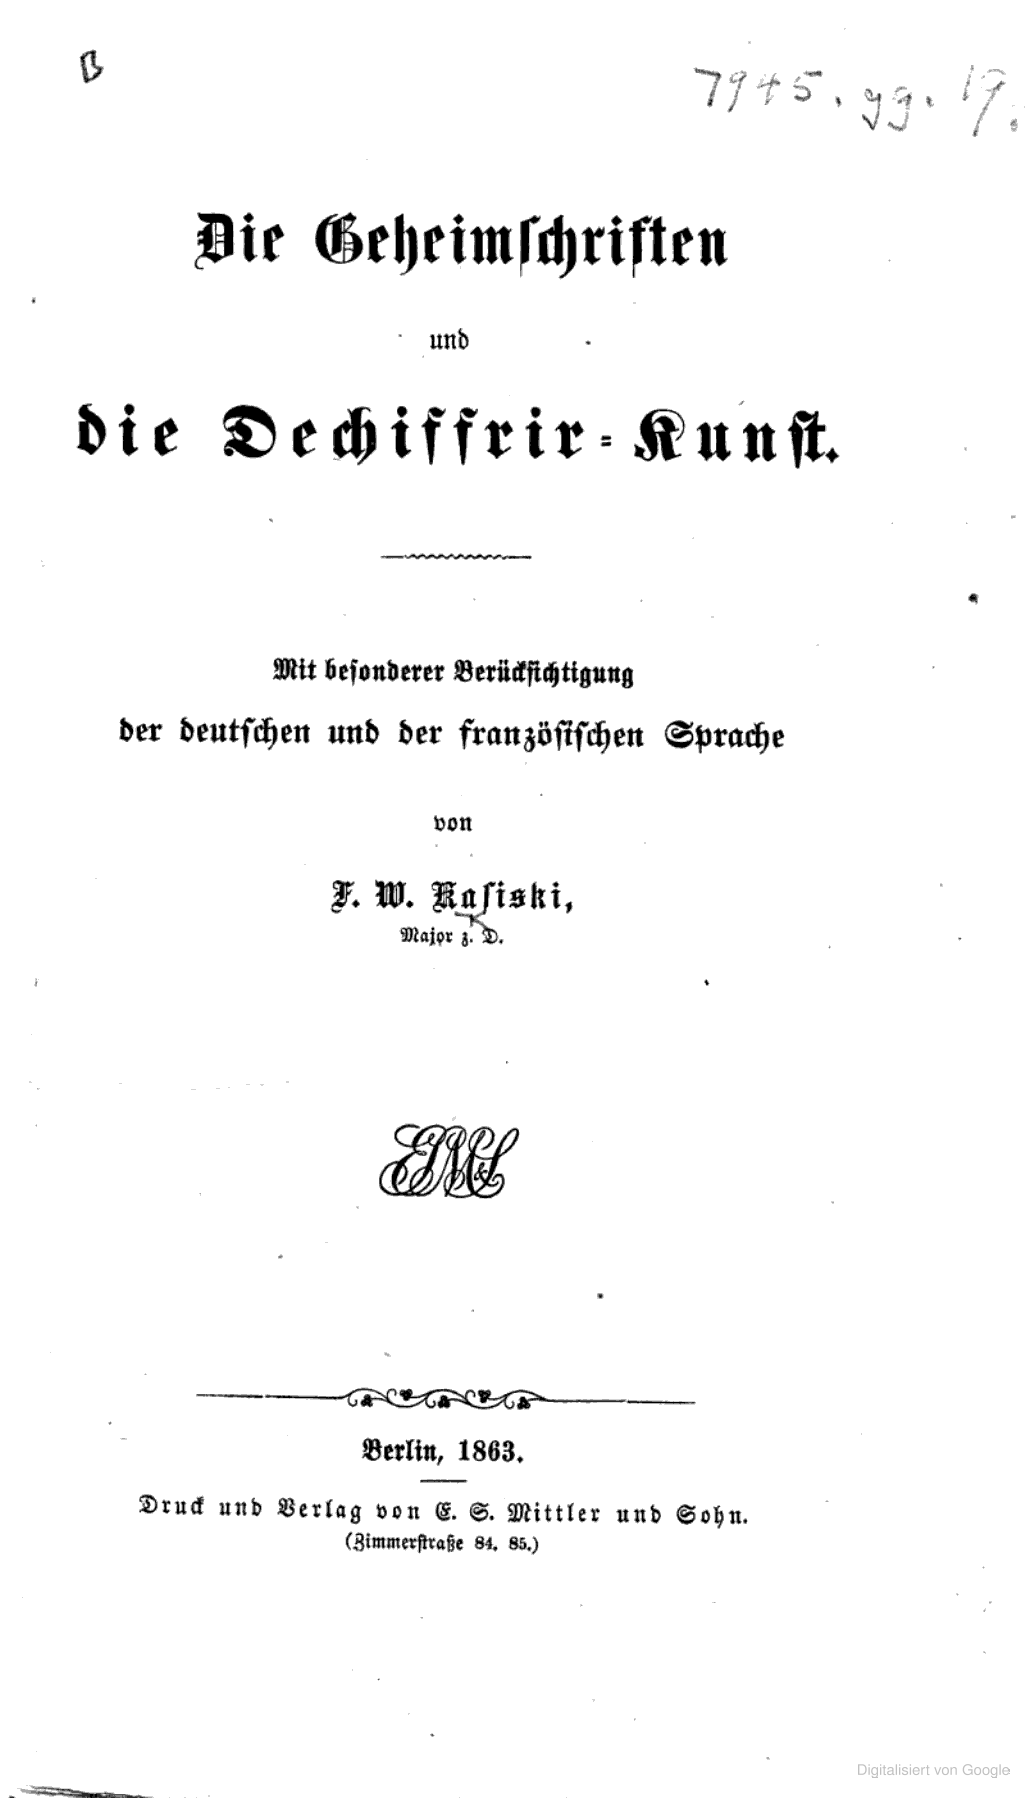
\includegraphics[width=.4\linewidth]{Grundlagen_Info/03_Kryptologie/Figures/kasiski-book}
	\caption{Umschlag des Buches \enquote{Die Geheimschriften und die Dechiffrir-Kunst} von Friedrich Kasiski (1863, \href{https://books.google.de/books?id=fB5dAAAAcAAJ}{Quelle})}
	\label{fig:kasiski-test-book}
\end{figure}

Die Grundidee hinter dem Kasiski-Test ist: Wenn ein Wort oder ein Wortteil im Klartext mehrmals vorkommen, so wird dieser möglicherweise auch im Kryptotext mehrmals vorkommen. Wenn beispielsweise die Buchstaben \enquote{\texttt{DIE}} mehrmals mit dem Schlüssel \enquote{\texttt{KEY}} verschlüsselt werden, dann wird der Text \enquote{\texttt{LIV}} mehrmals im Geheimtext auftauchen. Wenn das Wort \enquote{\texttt{DIE}} also zweimal im Klartext vorkommt \textbf{und} auf denselben Schlüsselteil (\enquote{\texttt{KEY}}, \enquote{\texttt{EYK}} oder \enquote{\texttt{YKE}}) fällt, wird z.B. \enquote{\texttt{LIV}} auch zweimal im Kryptotext gleich verschlüsselt sein.

Wenn wir also im Kryptotext nach wiederholten Sequenzen suchen, können wir daraus die Schlüssellänge ableiten.

\begin{myexample}\label{ex:kasiskiTest}
In folgendem Beispiel ist der Klartext auf der ersten Zeile. Der Schlüssel ``\text{CODE}'' wird verwendet, um den Gemeimtext (auf der dritten Zeile) zu erzeugen:

\texttt{M\gold{EIN}KL\red{EIN}ERREIMSCH\red{EIN}TK\green{EIN}ERZUS\green{EIN}}

\texttt{C\gold{ODE}CO\red{DEC}ODECODECO\red{DEC}OD\green{ECO}DECOD\green{ECO}}

\texttt{O\annotKasiski{Gold}{S}{LR}{2}MZ\annotKasiski{red}{H}{MP}{7}SUVGWPWEV\annotKasiski{red}{H}{MP}{19}HN\annotKasiski{ForestGreen}{I}{KB}{24}HVBIV\annotKasiski{ForestGreen}{I}{KB}{32}\\[.5cm]}

Der Kasiski-Test erlaubt uns, Hinweise auf die Schlüssellänge zu erhalten, ohne den Schlüssel zu kennen:
\begin{itemize}
	\item Die Sequenzen \enquote{\texttt{HMP}} und \enquote{\texttt{IKB}} erscheinen jeweils zweimal im Geheimtext.
	\item Die Sequenz \texttt{HMP} befindet sich an den Positionen 7 und 19. Die Differenz zwischen diesen Positionen beträgt 12, was sich als $2\times2\times3$ in Primfaktoren zerlegen lässt.
	      \begin{tcolorbox}
		      $\mathbf{\underset{\text{Position 1 \texttt{HMP}}}{7}+\underset{\text{Codewort-Länge!}}{\blue{4}}\times \underset{\text{Anzahl Codewörter}}{3} = \underset{\text{Position 2 \texttt{HMP}}}{19}}$
	      \end{tcolorbox}
	\item Die Sequenz \texttt{IKB} befindet sich an den Positionen 24 und 32. Die Differenz zwischen diesen Positionen beträgt 8, was sich als $2\times2\times2$ faktorisieren lässt.
	      \begin{tcolorbox}
		      $\mathbf{\underset{\text{Position 1 \texttt{IKB}}}{24}+\underset{\text{Codewort-Länge!}}{\blue{4}}\times \underset{\text{Anzahl Codewörter}}{2} = \underset{\text{Position 2 \texttt{IKB}}}{32}}$
	      \end{tcolorbox}
	\item Die Schlüssellänge könnte, sofern man nur den Abstand zwischen den beiden \texttt{HMP} betrachtet, theoretisch auch 12 sein. Dann würden allerdings die beiden \texttt{IKB} nicht auf denselben Schlüsselteil fallen. Daher ist dies nicht möglich.
	\item Den Primfaktoren $2\times2\times3$ und $2\times2\times2$ ist der Teil $2\times2$ gemeinsam, was darauf hindeutet, dass die \textbf{Schlüssellänge 4} sein könnte.
\end{itemize}
\end{myexample}

\clearpage  % using clearpage to enable printing out the exercise on just one page
\begin{myexercise}[Vigenère knacken bei bekannter Schlüssellänge (zu dritt)]\label{ex:vigKasiski}
	Finden Sie den Klartext für folgende Nachricht heraus, wenn Sie wissen, dass der Text mit Vigenère verschlüsselt worden ist. Wenden Sie den Kasiski-Test an!

	\begin{alltt}
UEU\underline{I}\underline{O}\underline{O}CEU\(\underset{\makebox[\widthof{\texttt{X}}][c]{\footnotesize\texttt{\red{10}}}}{\texttt{\red{D}}}\)IW\underline{I}\underline{O}\underline{O}WRRC\(\underset{\makebox[\widthof{\texttt{X}}][c]{\footnotesize\texttt{\red{20}}}}{\texttt{\red{L}}}\)WVUQURRCL\(\underset{\makebox[\widthof{\texttt{X}}][c]{\footnotesize\texttt{\red{30}}}}{\texttt{\red{W}}}\)VNDTHXETH\(\underset{\makebox[\widthof{\texttt{X}}][c]{\footnotesize\texttt{\red{40}}}}{\texttt{\red{E}}}\)RRCFKRTWV\(\underset{\makebox[\widthof{\texttt{X}}][c]{\footnotesize\texttt{\red{50}}}}{\texttt{\red{S}}}\)FYOQRNJJT\(\underset{\makebox[\widthof{\texttt{X}}][c]{\footnotesize\texttt{\red{60}}}}{\texttt{\red{G}}}\)\\[.5cm]\rule{\linewidth}{1pt}
RSVUAV\underline{I}\underline{O}\underline{O}\(\underset{\makebox[\widthof{\texttt{X}}][c]{\footnotesize\texttt{\red{70}}}}{\texttt{\red{C}}}\)EQEIHRUIY\(\underset{\makebox[\widthof{\texttt{X}}][c]{\footnotesize\texttt{\red{80}}}}{\texttt{\red{O}}}\)HITQLNJZN\(\underset{\makebox[\widthof{\texttt{X}}][c]{\footnotesize\texttt{\red{90}}}}{\texttt{\red{J}}}\)VSEVRJRUI\(\underset{\makebox[\widthof{\texttt{X}}][c]{\footnotesize\texttt{\red{100}}}}{\texttt{\red{L}}}\)NGUEU\underline{I}\underline{O}\underline{O}C\(\underset{\makebox[\widthof{\texttt{X}}][c]{\footnotesize\texttt{\red{110}}}}{\texttt{\red{E}}}\)UDIW\underline{I}\underline{O}\underline{O}WH\(\underset{\makebox[\widthof{\texttt{X}}][c]{\footnotesize\texttt{\red{120}}}}{\texttt{\red{R}}}\)\\[.5cm]\rule{\linewidth}{1pt}
VRWVAXWZX\underline{\(\underset{\makebox[\widthof{\texttt{X}}][c]{\footnotesize\texttt{\red{130}}}}{\texttt{\red{I}}}\)}\underline{O}\underline{O}CEQ\underline{I}\underline{O}\underline{O}W\(\underset{\makebox[\widthof{\texttt{X}}][c]{\footnotesize\texttt{\red{140}}}}{\texttt{\red{A}}}\)WDEWVAXWU\(\underset{\makebox[\widthof{\texttt{X}}][c]{\footnotesize\texttt{\red{150}}}}{\texttt{\red{Q}}}\)UWRCLWVDL\(\underset{\makebox[\widthof{\texttt{X}}][c]{\footnotesize\texttt{\red{160}}}}{\texttt{\red{V}}}\)NDVCKJTHE\(\underset{\makebox[\widthof{\texttt{X}}][c]{\footnotesize\texttt{\red{170}}}}{\texttt{\red{T}}}\)DXEYFMUFL\(\underset{\makebox[\widthof{\texttt{X}}][c]{\footnotesize\texttt{\red{180}}}}{\texttt{\red{O}}}\)\\[.5cm]\rule{\linewidth}{1pt}
VRQZCKKSP\(\underset{\makebox[\widthof{\texttt{X}}][c]{\footnotesize\texttt{\red{190}}}}{\texttt{\red{V}}}\)HUYOHIEQ\\[.5cm]\rule{\linewidth}{1pt}
	\end{alltt}
	\normalsize

	\textbf{Anleitung:}
	\begin{itemize}
		\item Die Position an allen 10, 20, 30 etc. Buchstaben sind oben bereits markiert, ebenso wie Vorkommnisse des Trigramms \underline{\texttt{IOO}}.
		\item Auf separatem Blatt:
		      \begin{enumerate}
			      \item Notieren Sie sich die \textbf{Anfangspositionen} aller Trigramme \underline{\texttt{IOO}}.
			      \item Berechnen Sie die \textbf{Abstände} zwischen den Anfangspositionen. Es reicht, wenn Sie nur die Abstände aller Anfangspositionen von \underline{IOO} zum ersten Trigramm \underline{IOO} an Position 4 berechnen.
			      \item Zerlegen Sie die Abstände zwischen den Trigrammen in \textbf{Primfaktoren}.
			      \item Finden Sie den \textbf{grössten gemeinsamen Teiler} dieser Primfaktoren, um die Schlüssellänge zu erraten.
		      \end{enumerate}
		\item Wenn Sie die Schlüssellänge haben, färben Sie den Text abwechslungsweise ein, wie in \cref{ex:vigHaufigkeitGruppen}. Teilen Sie sich zu dritt auf, so dass jede Person eine Gruppe von Buchstaben entschlüsselt (gleich wie in \cref{ex:vigHaufigkeitGruppen}).
		\item \textbf{Tipp}: Der letzte Teil des Schlüssels ist ``\texttt{D}''. Der Schlüssel ergibt ein Wort. Entschlüsseln Sie den Text nun mit der \href{https://inventwithpython.com/cipherwheel/}{Caesar-Drehscheibe}! Entschlüsseln Sie zuerst nur die erste Zeile, um zu überprüfen, ob ihr Schlüssel stimmt und zu einem sinnvollen Text führt.
	\end{itemize}
	\begin{myanswer}
		Positionen der Anfangs-Trigramme: 4, 13, 67, 106, 115, 130, 136. Abstände und Primfaktoren sind beispielsweise:
		\begin{align*}
			13-4  & = & 9   & = & 3\times3                \\
			67-4  & = & 63  & = & 3\times3\times7         \\
			106-4 & = & 102 & = & 2\times3\times17        \\
			115-4 & = & 111 & = & 3\times37               \\
			130-4 & = & 126 & = & 2\times3\times3\times7  \\
			136-4 & = & 132 & = & 2\times2\times3\times11 \\
		\end{align*}

		Man erkennt, dass die Primzahl 3 bei jeder Differenz vorkommt, also ist der Schlüssel vermutlich 3. Wir können nun wie in \cref{ex:vigHaufigkeitGruppen} verfahren, um den Text zu knacken. Mittels Häufigkeitsanalyse (und etwas Ausprobieren mit dem häufigsten, zweithäufigsten Buchstaben etc.) finden wir folgenden Schlüssel heraus: \texttt{RAD}. Somit kann der Klartext nun entziffert werden:
		
		\colorstring[ForestGreen,RoyalBlue,Crimson]{DERROLLERMITROLFROLLTEUNDROLLTENACHUNTENROLFHATTESCHONANGSTDASSDASROLLENNIEAUFHOERTNUNGINGESBERGAUFUNDDERROLLERMITROLFHOERTEAUFZUROLLENROLFATMETEAUFUNDWOLLTEDIENAECHSTENTAGEVOMROLLERNICHTSMEHRHOEREN}
	\end{myanswer}
\end{myexercise}

\begin{myexercise}
	Finden Sie die Schlüssellänge für folgenden Vigenère-Text heraus, indem Sie den Kasiski-Test anwenden:

	\texttt{\colorstring[black]{CMFBAMXPESRGILLDMNCEDMTKEHRPVFEIOKLHGIVSJYSQZDMUXYLRBJITQNZTDMOVMUMFCSDMUZGDRTTHVISGUMOURNFICFTRMFSEQIJKESJBVHHKFLNCPFINVMMCIFIKLGDRECIBLFRUEIJEEFCNEARMBCELEULRTREUALMURUEHJVAMJPIDDVVEGDRFZNDWIFCGWDYUKWULDHYNJVNVOVBDREVRESFIDDVVEGHRUVLKILKUDPMVREEFYIFOFZTDRVEDEISKIFOFZTDRXVRCIOUIDNVXEMHMZCGIORUBLJEIGVFIPDVTFEMPJTHDRFETVMDBLTRHLNSISJTTIUQTHQWFRKMFXEMHFELDMUSIKHTZNCDJVLDYOUWDVUVFDWUXEGEMKEMRBTHCIOVNRMDYDHITTHTPBEGDLPVRHKFEIMMIIEQXBVGKMDYEMESSEHXSZCGXFEERFJCDDXALDDQEZEFVVEDKEHVFTISUIDFFIPQYFWUMKVESDVFJTTRTLNCJVVRCM}}

	Verwenden Sie dazu folgendes Online-Tool: \url{https://cryptbreaker.marcwidmer.xyz/solve}
	\begin{enumerate}
		\item Verwenden Sie das Analyse-Werkzeug \enquote{Kasiski-Analyse}, um die Abstände der sich wiederholenden Sequenzen der Länge 4 zu bestimmen.
		      \begin{itemize}
			      \item Notieren Sie sich die Positionen und Abstände der sich wiederholenden Sequenzen der Länge 4.
			      \item Zerlegen Sie die Abstände in Primfaktoren.
			      \item Finden Sie den grössten gemeinsamen Teiler der Abstände, um die Schlüssellänge zu erraten.
		      \end{itemize}
		\item Überprüfen Sie Ihre Vermutung, indem Sie im Analyse-Werkzeug die Häufigkeitsanalyse mit der Schrittweite (\textit{stride}) gleich der vermuteten Schlüssellänge durchführen.
		\item Entschlüsseln Sie den Text mit dem \enquote{Vigenère}-Entschlüsslungswerkzeug.
	\end{enumerate}

	\begin{myanswer}
		\begin{enumerate}
			\item Wir beobachten folgende Positionen und Abstände bei den Zeichenfolgen der Länge 4:
			      \begin{itemize}
				      \item \texttt{XEMH}: 283, 348 (Abstand 65) $\rightarrow$ $5\times13$
				      \item \texttt{IDDV}: 223, 178 (Abstand 45) $\rightarrow$ $3\times3\times5$
			      \end{itemize}
			      Bereits aus diesen beiden Zeichenfolgen erkennen wir einen gemeinsamen Teiler von 5 und somit eine mögliche Schlüssellänge von 5.
			\item Die Häufigkeitsanalyse mit Schrittweite 5 bestätigt unsere Vermutung, da die Häufigkeitsverteilung pro Gruppe stark von der Gleichverteilung abweicht.
			\item Mit dem Schlüssel \texttt{ZEBRA} können wir den Text entschlüsseln und enthalten einen Ausschnitt des \href{https://www.ksimlee.ch/schule/leitbild/}{Leitbilds der Kantonsschule im Lee}.
		\end{enumerate}
	\end{myanswer}
\end{myexercise}

\begin{myexercise}
	\begin{enumerate}
		\item Erklären Sie kurz: Dopplungen im Klartext (z.B. \enquote{EIN}) führen nicht unbedingt zu Dopplungen im Geheimtext.
		\item Erklären Sie kurz: Dopplungen im Geheimtext müssen nicht in jedem Fall aus Dopplungen im Klartext stammen; sie können auch zufällig entstehen.
	\end{enumerate}

	\begin{myanswer}
		Kurzbegründungen:
		\begin{itemize}
			\item Bei polyalphabetischer Verschlüsselung werden gleiche Trigramme an verschiedenen Textpositionen oft mit verschiedenen Schlüsselzeichen verschlüsselt, sodass Wiederholungen im Klartext nicht zwangsläufig gleiche Geheimtrigramme ergeben (s. z.B. \cref{ex:kasiskiTest}).
			\item Geheimtext-Dopplungen können aber auch zufällig entstehen (z.B. ``\texttt{OML}''), wenn verschiedene Klartextfolgen unter unterschiedlichen Schlüsselteilen zufällig identische Geheimfolgen produzieren. Beispiel:
			      \begin{itemize}
				      \item Klartext: \texttt{EIN} mit Schlüsselteil \texttt{KEY} $\rightarrow$ Geheimtext: \texttt{OML}
				      \item Klartext: \texttt{KOB} mit Schlüsselteil \texttt{EYK} $\rightarrow$ Geheimtext: \texttt{OML}
			      \end{itemize}
		\end{itemize}
	\end{myanswer}
\end{myexercise}

\begin{mychallenge}
	Lösen Sie den Kasiski-Test online:
	\qrcode[height=2cm]{https://www.dominikus-gymnasium.de/kasiski-test-spiel.html}
\end{mychallenge}

\subsubsection{Bestimmung der Schlüssellänge: Friedman'sche Charakteristik}

Eine weitere Möglichkeit, die Schlüssellänge zu erraten, besteht in der Verwendung der sogenannten Friedman'schen Charakteristik.

William Friedman (1891-1969) war ein russisch-amerikanischer Kryptologe und Pionier auf dem Gebiet der Kryptoanalyse (siehe \cref{fig:william-friedman}). Kurz vor dem Ausbruch des zweiten Weltkriegs gründete er den Signals Intelligence Service (SIS), eine Geheimabteilung des US-Militärs zur Entzifferung feindlicher Codes und Geheimschriften.

\begin{figure}[H]
	\centering
	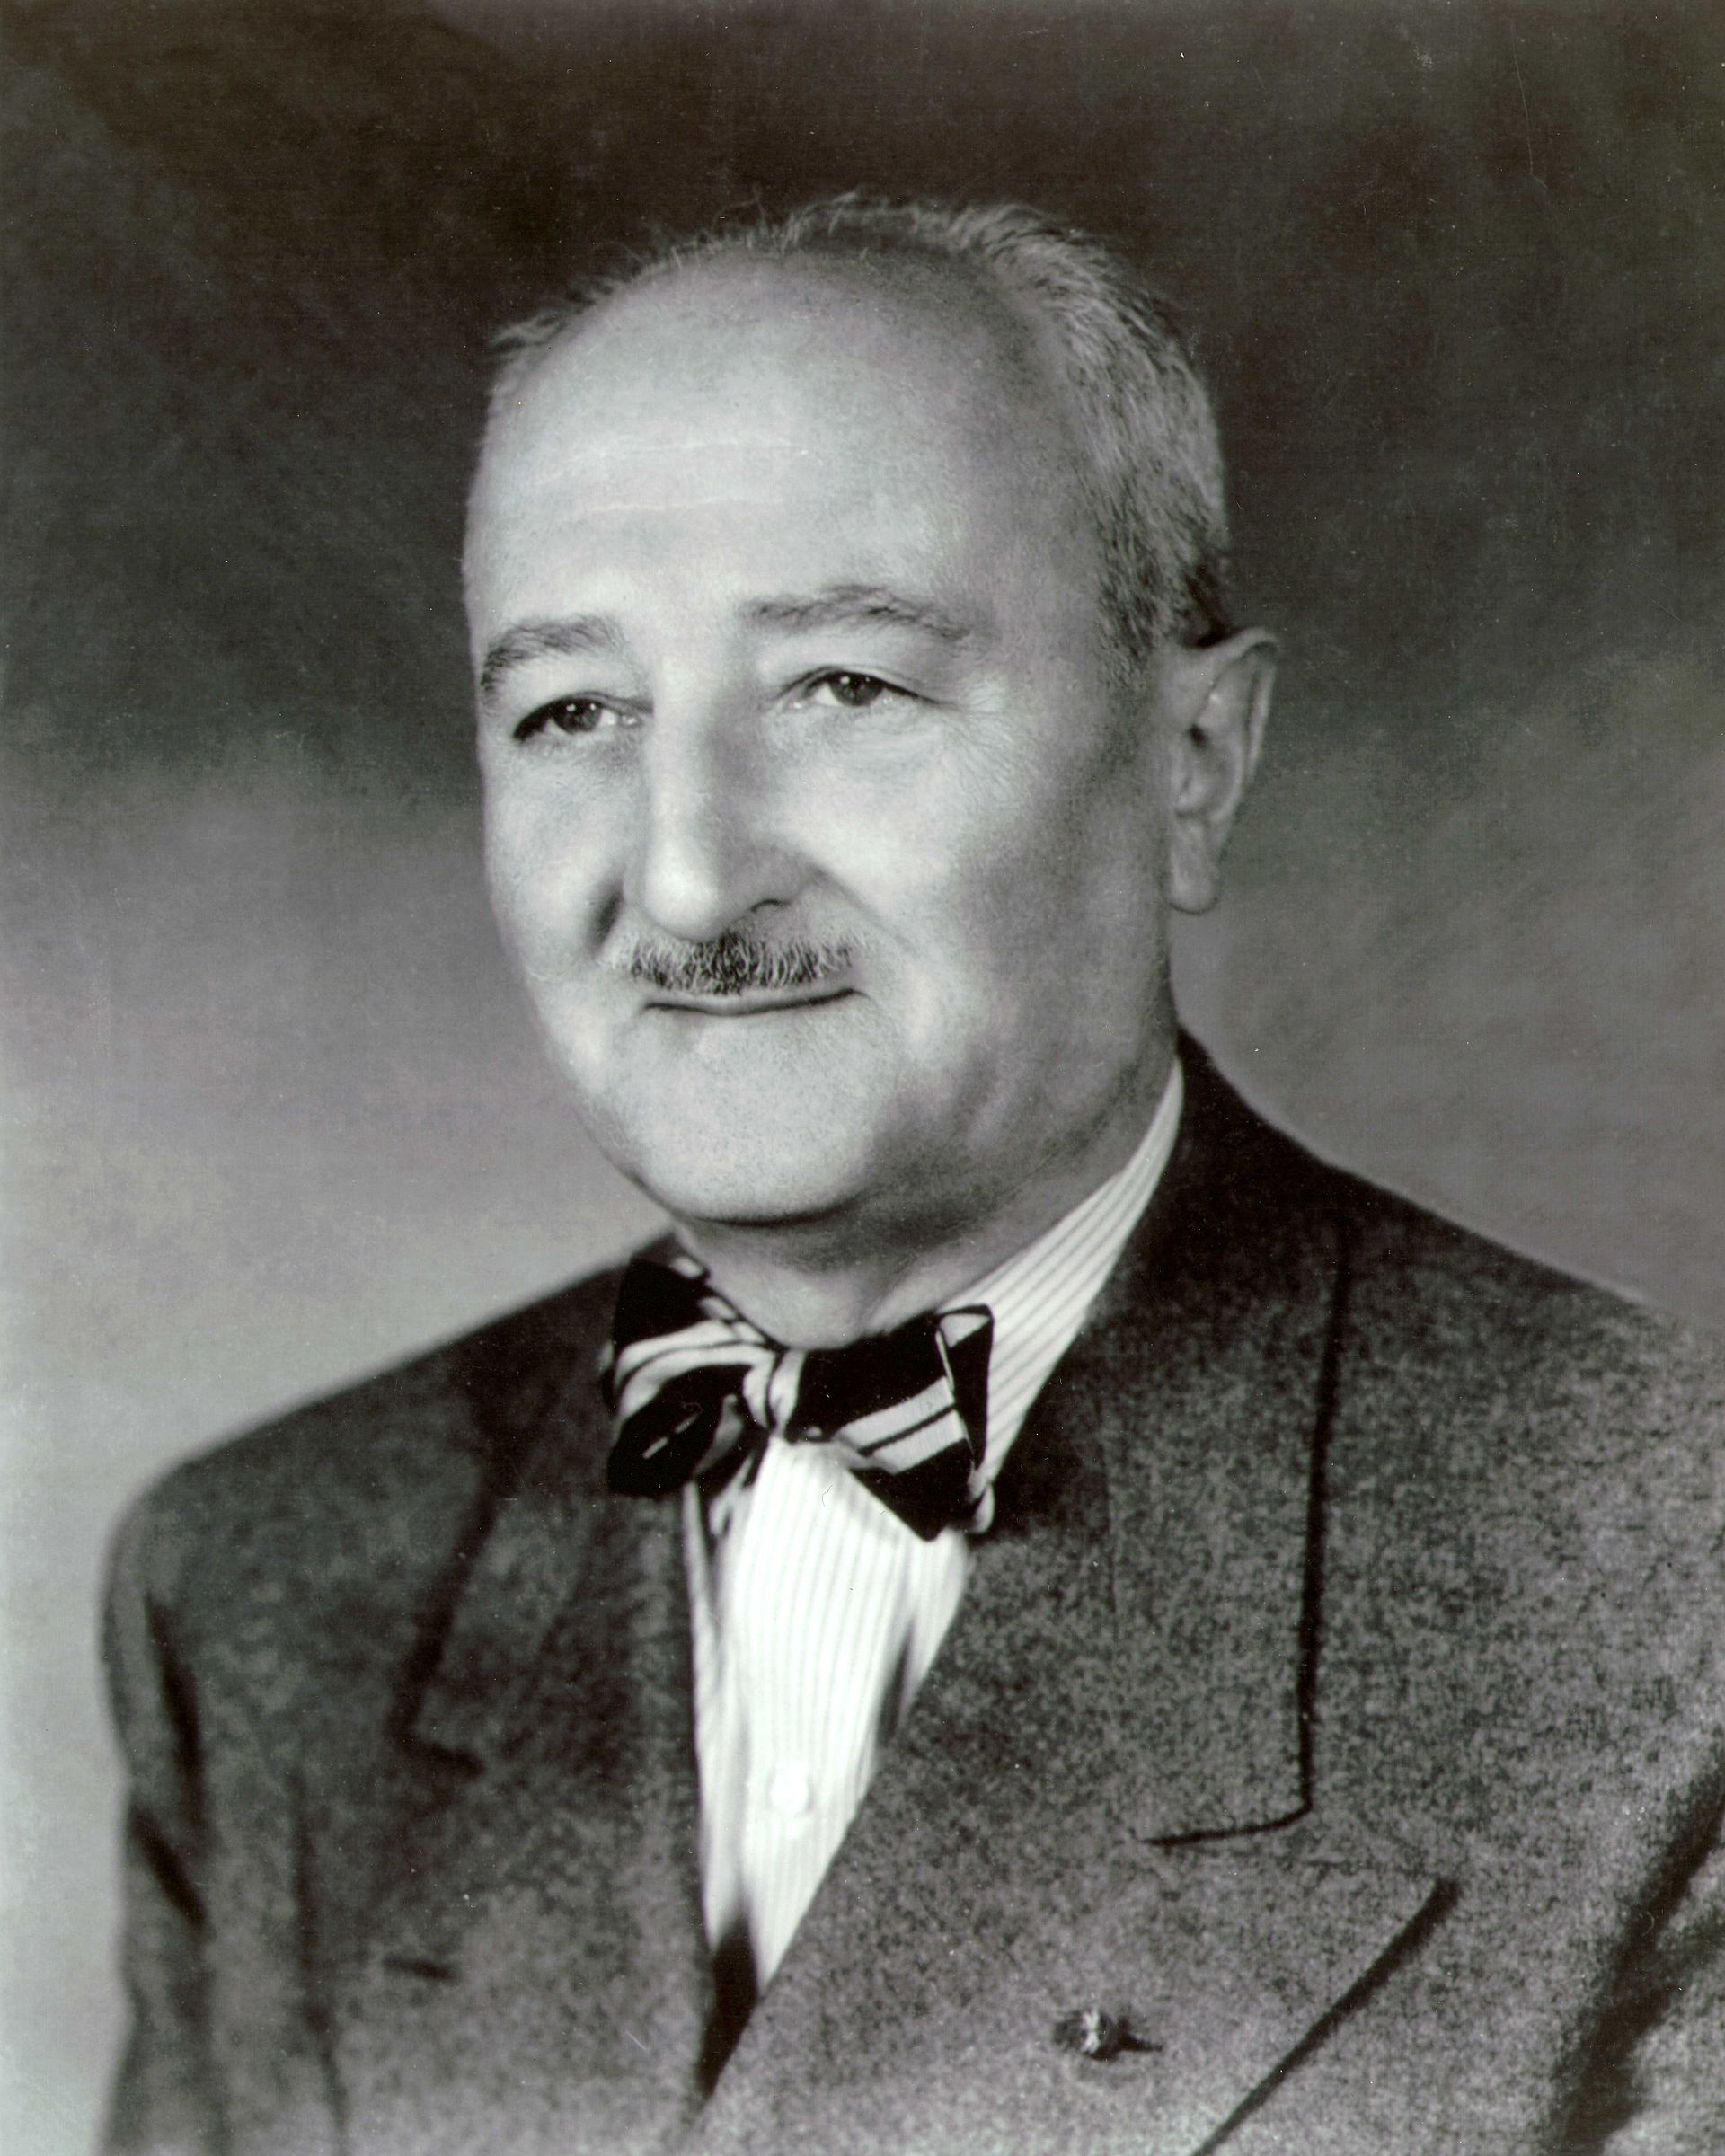
\includegraphics[width=.3\linewidth]{Grundlagen_Info/03_Kryptologie/Figures/William-Friedman.jpg}
	\caption{William Friedman (\href{https://de.wikipedia.org/wiki/William\_Friedman\#/media/Datei:William-Friedman.jpg}{Quelle})}
	\label{fig:william-friedman}
\end{figure}

Die Friedman'sche Charakteristik macht sich zunutze, dass Buchstaben im Klartext ungleich verteilt sind. Falls jeder Buchstabe gleich häufig vorkommen würde, wäre die erwartete Häufigkeit jedes Buchstabens genau $1/26$. In keiner natürlichen Sprache besitzen alle Buchstaben dieselbe relative Häufigkeit. Die Häufigkeitsverteilung der Buchstaben in deutschen Texten haben wir bereits in \cref{tab:alle-haeufigkeiten} gesehen. Die relative Häufigkeit des Buchstabens \enquote{E} in deutschen Texten ist beispielsweise ca. 17.4\%. Die relative Häufigkeit eines Buchstabens $\square$ in einem Text $T$ bezeichnen wir mit $h_\square(T)$.

Die Friedman'sche Charakteristik berechnet, wie ungleich alle Buchstaben in einem Text verteilt sind, indem sie die quadrierte Differenz der relativen Häufigkeit jedes Buchstabens zu $1/26$ berechnet. Diese quadrierten Abweichungen werden danach alle aufsummiert (siehe. \cref{eq:fc}).

\begin{myremark}
	Das Quadrieren der Abweichungen (Differenzen) hat zwei Effekte:
	\begin{itemize}
		\item Quadrate von reellen Zahlen sind sicherlich nicht negativ.
		\item Grosse Abweichungen von $1/26$ tragen aufgrund des Quadrierens überproportional zur Summe (zur Friedmansch'schen Charakteristik) bei.
	\end{itemize}
\end{myremark}

\begin{align}\label{eq:fc}
	FC(T) & =\lr{h_A(T)-\frac{1}{26}}^2+\lr{h_B(T)-\frac{1}{26}}^2+\ldots+\lr{h_Z(T)-\frac{1}{26}}^2 \\
	      & =\sum_{\Delta\in \text{Alphabet}}\lr{h_\Delta(T)-\frac{1}{26}}
\end{align}

Eine stark ungleiche Verteilung von Buchstaben in einem Text $T$ führt also zu einer hohen Friedman'schen Charakteristik $FC(T)$, währenddem gleichmässig verteiltere Buchstaben im Text $T$ zu einer tieferen $FC(T)$ führen. Deutschsprachige (Klar-)Texte haben durchschnittlich etwa einen Wert von 3.8\% (0.038) (siehe \cref{fig:vig-subgroup-1-avg}).

\begin{figure}[H]
	\centering
	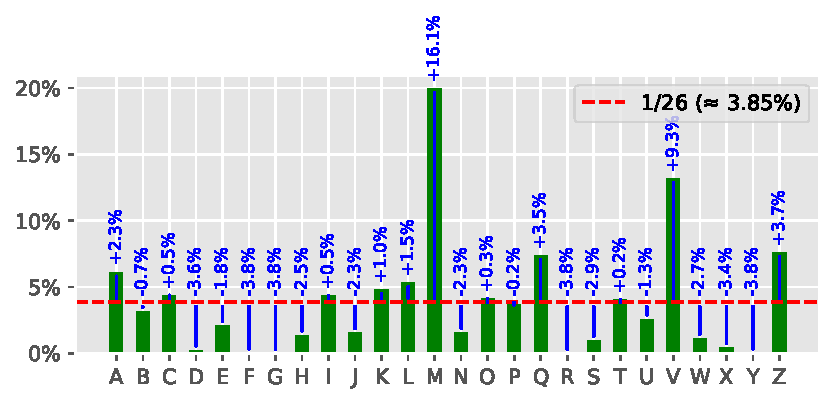
\includegraphics[width=.8\linewidth]{Grundlagen_Info/03_Kryptologie/Figures/vigenere-len3-group1-avg}
	\caption{Buchstabenhäufigkeit in einem mit Caesar verschlüsselten Text, im Vergleich zur Gleichverteilung von Buchstaben}
	\label{fig:vig-subgroup-1-avg}
\end{figure}

Je grösser die blauen Pfeile in \cref{fig:vig-subgroup-1-avg}, desto höher die Friedman'sche Charakteristik.

Wir können nun folgenden \textit{Brute-Force}-Ansatz verwenden, um die Schlüssellänge mit der Friedman'schen Charakteristik zu bestimmen:

\begin{itemize}
	\item Alle möglichen Schlüsselwortlängen von 1 bis zu einer beliebig gewählten Zahl $n$ ausprobieren, wobei $n$ praktisch nie über 10 gewählt wird.
	\item Buchstaben jeweils in Gruppen unterteilen:
	      \begin{itemize}
		      \item \textbf{2 Gruppen}: \texttt{\colorstring[ForestGreen,RoyalBlue]{MUZ KJL QPA WJU MHY IIL LCZ AUP MRL ZHL SVC
				            MTZ BCU LGU PCI MPD QGT IPC QIL VGY MGU BUJ
				            PNB MUZ MNA PGY HNP KJL OTH BWS IVP WPK IHB}}
		            \begin{figure}[H]
			            \centering
			            \foreach \i/\groupColor in {1/ForestGreen,2/RoyalBlue} {
					            \begin{subfigure}{.24\textwidth}
						            \centering
						            \includegraphics[width=\textwidth]{Grundlagen_Info/03_Kryptologie/Figures/vigenere-len2-group\i}
						            \caption{\textcolor{\groupColor}{Gruppe \i}}
					            \end{subfigure}}
			            \caption{Buchstaben-Häufigkeiten und $FC_T$ für Schlüsssellänge=2}
		            \end{figure}

		      \item \textbf{3 Gruppen}: \texttt{\colorstring[ForestGreen,RoyalBlue,Crimson]{MUZ KJL QPA WJU MHY IIL LCZ AUP MRL ZHL SVC
				            MTZ BCU LGU PCI MPD QGT IPC QIL VGY MGU BUJ
				            PNB MUZ MNA PGY HNP KJL OTH BWS IVP WPK IHB}}
		            \begin{figure}[H]
			            \centering
			            \foreach \i/\groupColor in {1/ForestGreen,2/RoyalBlue,3/Crimson} {
					            \begin{subfigure}{.24\textwidth}
						            \centering
						            \includegraphics[width=\textwidth]{Grundlagen_Info/03_Kryptologie/Figures/vigenere-len3-group\i}
						            \caption{\textcolor{\groupColor}{Gruppe \i}}
					            \end{subfigure}}
			            \caption{Buchstaben-Häufigkeiten und $FC_T$ für Schlüsssellänge=3}
		            \end{figure}
		      \item \textbf{4 Gruppen}: \texttt{\colorstring[ForestGreen,RoyalBlue,Crimson,LightSlateBlue]{MUZ KJL QPA WJU MHY IILLCZ AUP MRL ZHL SVC MTZ BCU LGU PCI MPD QGT IPC QIL VGY MGU BUJ PNB MUZ MNA PGY HNP KJL OTH BWS IVP WPK IHB}}
		            \begin{figure}[H]
			            \centering
			            \foreach \i/\groupColor in {1/ForestGreen,2/RoyalBlue,3/Crimson,4/LightSlateBlue} {
					            \begin{subfigure}{.24\textwidth}
						            \centering
						            \includegraphics[width=\textwidth]{Grundlagen_Info/03_Kryptologie/Figures/vigenere-len4-group\i}
						            \caption{\textcolor{\groupColor}{Gruppe \i}}
					            \end{subfigure}}
			            \caption{Buchstaben-Häufigkeiten und $FC_T$ für Schlüsssellänge=4}
		            \end{figure}
		      \item etc, bis zu Schlüssellänge = n
	      \end{itemize}
	\item Für jede der Schlüssellängen: Durchschnittliche $FC(T)$ für alle Gruppen berechnen.
	\item Wenn die richtige Schlüssellänge (oder ein Vielfaches davon) gewählt wurde, sollte $FC(T)$ höher sein.
\end{itemize}

Die durschschnittliche Friedman'sche Charakteristik für jede der getesteten Schlüssellängen ist gezeigt in \cref{fig:fc}.

\begin{figure}[H]
	\centering
	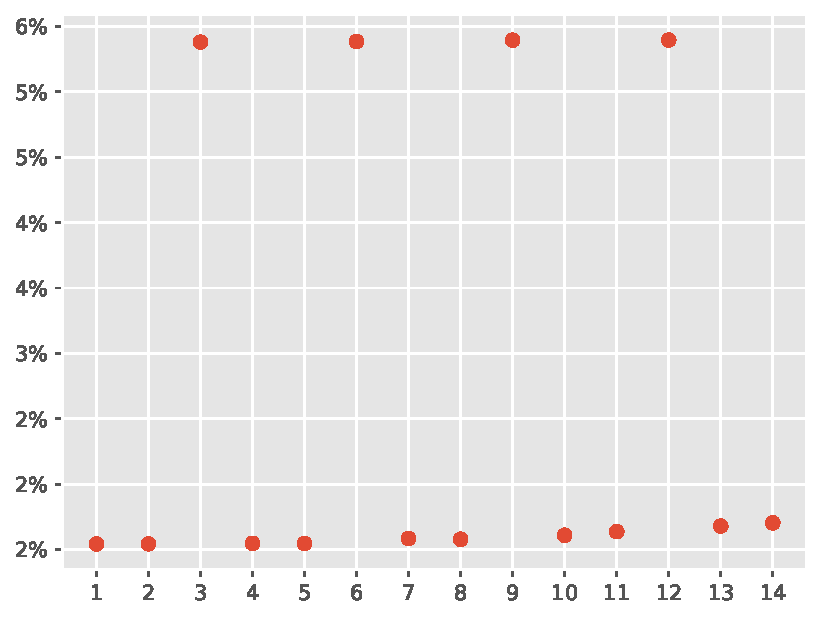
\includegraphics[width=.6\linewidth]{Grundlagen_Info/03_Kryptologie/Figures/friedman}
	\caption{Durchschnittliche Friedman'sche Charakteristik für jede Schlüssellänge}
	\label{fig:fc}
\end{figure}

Aus \cref{fig:fc} lässt sich ablesen, dass die Schlüssellänge vermutlich 3 sein muss, da bei jedem Vielfachen der Schlüssellänge 3 die durchschnittliche Friedman'sche Charakteristik höher ist als für die restlichen Schlüssellängen. Ab nun lässt sich gleich vorgehen wie in \cref{subsubsec:vigHack} beschrieben, um den Text zu entschlüsseln.

\begin{myexercise}
	Berechnen Sie die Friedman'sche Charakteristik für folgende beide Texte von Hand:

	\texttt{\colorstring[black]{PAPPERLAPAPP}}

	\texttt{\colorstring[black]{BACKSTEIN}}

	Wie interpretieren Sie die beiden Zahlen?
	\begin{myanswer}
		Die Friedman'sche Charakteristik beträgt 29.5\% und 7.3\%, respektive. Wie sie sehen, ist die Friedmansch'e Charakteristik höher für Texte, bei denen jeder Buchstabe relativ häufiger vorkommt.
	\end{myanswer}
\end{myexercise}

\begin{myexercise}
	Für welche Buchstabenverteilung sollte die Friedman'sche Charakteristik höher sein: \cref{fig:langer-text-vig-caesar}, (a) oder (b)?
	\begin{myanswer}
		$FC(T)$ sollte für \cref{fig:langer-text-vig-caesar} (a) höher sein, da die durchschnittliche relative Häufigkeit der Buchstaben im Kryptotext ungleicher ist.
	\end{myanswer}
\end{myexercise}


\begin{myexercise}

	Kopieren Sie den folgenden Kryptotext und versuchen Sie, ihn mit dem \href{https://cryptbreaker.marcwidmer.xyz}{Analysetool} zu entziffern, indem Sie zuerst das Tool ``Friedman'' und danach das Tool ``Frequency'' verwenden. Wie lautet der Schlüssel?

	\texttt{\colorstring[black]{FZNZKVEDZFCRRZVFZTZFLVIOVBKMZWOVGVBAVSZSMVEDBHVNJANVNBZFZCCRFESPSTJEITSLECZJEGNAPIGZBEZEDQIDIOUBEZZAIVRUSOXEIWFJSZWDYBDBBCLZWOLNYTSVUZAJTHHSJEENZFSEIGJEDDSTVRBSHVNYRJVFPSSJOGQIVSZSMVNBSTTHVTGVNDGUNIZRJVMZWOVIXVCZNNCHCUZQLCIXVNVIIPFJTZFTFGVBAZNYSNXEAIFYLZJPERPVJXEHRBJEDBWVRNIOBEIRBJSHSJEEFIOJTYOSLNOSSCEDRFKIXVLFEIBUVJZHAKNDQIKZZWDYNZBOZCCHFZNZBTKRDQILNYPJENDSFZNBFPVSNSSVRHOMVRBSXVSZBBCSDBEZENSORUBSOSLDQLVNRSOEDVGMZEWSURLPANZCCRBDPAHVEDYWFYOCSTFNISBEDZFPSEMTMREXVFUEMIOUUMQIURDBHCIXVFEFDBTKEMBJJMZWOVSROMUENFVYTPBEEUMSJEZZZOVSOFBYLZBTZCCWOUANWOEEMSIVIGWHKUHGUVHGSOZCCRBENDAIFHZBHIANSBDFVZMVNYSOSAXVFCIZUFLNYBBVHZFBEDZFFIDZHBLSZBEDAIBJXFVZUZGZUSRENQIVNHWSDEMYXLEMRJXWZFEVNRSOEIXVERSRWNDEGBEVRFZFZNZBXVLONXZSXVFEHVZNVNYWFLNUOFYLDUFEUISSXRPSOULDQIVNBSTKAGHFEDZFXLEMADYEIRFIMPSDBCCSOEAZVFIAIAFZNZAIVRUSOWUZVMVUIRGLECZFUIZUFXEIKBITYSTRLGABVCCHJXEIRFIUIGORCCGFZNZACZLYSTTHPTERSRSIVNYSTRLGWFSEIRFEDZFVESDBFNIBSSNOIBFJCCKFSEIRUIAZUULNYSSYAZZUDEDBGIEPBENEIBTUAIBVDMZWOVAPUFEDVSNDEMHVEDYWFNEGHVDMDQIYEMIOUDZFIZMHSMXAINJEMZWOVRNSFCEMIIEWDSEZEBSTKAGHFZNZFHVLDSCKEIRBENNSIEEDQIDIXVPWTPBEUEIYFRCCYPVNIHFJTYIERSRWFUEMOVJDMIFTKZBLFEIBUVSORVUEHDBGIZFFUANSJEHVIDYEIKBJSJJPCLNCXRRHWOUIMZFSTYOTJENKVVRYSEVRNDJVGZZEVIISSJEZZFNIZRFZNZGFVLZWTKDZFTGIZUFCDZGVEEIRMZCCSOXOOHFJMZWOWRZIOUAWSSZCCUFYEYOSLEWSSQUBFVEDZWDYEMZJVGZIOKEMRFIGZKBCTYSSYEMFMZCCYFZTYWFJEMSSJCCSJEUIUFEEDBFNUIRFIBVFFYEDHFIKZWUYAOAFZNZUBEZZGFVLZSJEGZBPDMZBHCEDQIUEIGVVSNSOWRPSICIIUTDOMUFEDDSJTHHWUXAINFDHZFAVNBSOZENGFZCCPJEAGZFZNPBEWRZIFDIXVNVIISTCEWSOJIIRJVSZFHVGZBEUIZTVVRNCMTHZGFVLZBHVSXVBWFZBJJTRWFUIZAFZNZWDYBDBTFGGIFTKGWDYMZWOSENHFISJU}}

	\begin{myanswer}
		Der Schlüssel lautet ``\texttt{BRAVO}''.
	\end{myanswer}
\end{myexercise}

\begin{mychallenge}
	Berechnen Sie die Friedman'sche Charakteristik für folgenden Kryptotext:

	\texttt{\colorstring[black]{WORBHHHLUQOWWLDSYSQOWOUKSUDSNEGAAZAEBKISMRILHGPCVLIBZTRLMHYUSIEBILWJKULZSPGHCEFZUQOIQOWCOLSBCVKISZMOSFSZTNBHOSTSUFILHZPCVTEWUHSYZBVCVQEBLMKHHBNEBLIUAIVYDFHEBNTSBCVGUBBNUBTGVMCLGHPHFDAZAEBDISPHFHUGKUBZTIUDBLBSSUATIQOSHLIUAMSPNPBS}}

	Verwenden Sie dazu das Python-Skript auf Moodle, mit der Funktion \lstinline|def calculate_fc(text)|. Was entnehmen Sie der ihrer Antwort? Wurde der Text mit Caesar oder mit Vigenère verschlüsselt?

	\begin{myanswer}
		Der tiefe Wert von 1.4\% deutet darauf hin, dass der Text vermutlich mit Vigenère verschlüsselt wurde.
	\end{myanswer}
\end{mychallenge}

\begin{mychallenge}[Ver- und Entschlüsslung mit Python (zu zweit)]
	Laden Sie zuerst die Vigenère-Python-Dateien von Moodle herunter. Erstellen Sie danach einen Text in deutscher Sprache mit mindestens 1000 Zeichen, beispielsweise mittels folgender Webseite: \url{https://www.blindtextgenerator.de/}. Diesen werden Sie nun mit Python verschlüsseln.

	Teil 1: Verschlüsselung
	\begin{itemize}
		\item Verschlüsseln Sie Ihren Text, indem Sie die Funktion \lstinline|def vigenere(text, key, encrypt=True)| verwenden.
		\item Senden Sie Ihren verschlüsselten Text an Ihre(n) Partner(in), nicht aber den Schlüssel.
	\end{itemize}
	Teil 2: Entschlüsselung
	\begin{itemize}
		\item Sie erhalten den Kryptotext und müssen nun zuerst den Schlüssel herausfinden. Bestimmen Sie diese mithilfe der Friedman'schen Charakteristik, indem Sie die Funktion \lstinline|def get_friedman_vals(text, maxkeylen)| verwenden.
		\item Nachdem Sie die Schlüssellänge bestimmt haben, finden Sie innerhalb jeder Gruppe dem häufigsten Buchstaben. Dies können Sie mit der Funktion \lstinline|def show_letter_freq(text)| einfach umsetzen. Somit sollten Sie das Schlüsselwort herausfinden können.
		\item Entschlüsseln Sie nun den Kryptotext, indem Sie die Funktion \lstinline|def vigenere(text, key, encrypt=False)| verwenden.
	\end{itemize}

\end{mychallenge}

\begin{mychallenge}
	Lösen Sie drei ``beliebige Probleme'' auf der \href{https://cryptbreaker.marcwidmer.xyz}{Analyse-Webseite}.
\end{mychallenge}


\subsection{\texorpdfstring{\acrlong{OTP}}{OTP}}
Die One-Time-Pad-Verschlüsselungsmethode (\gls{OTP}, deutsch ``Einmalschlüssel-Verfahren'') funktioniert im Prinzip identisch wie die Vigenère-Methode, mit folgenden drei Unterschieden:
\begin{enumerate}
	\item Der Schlüssel besteht auf einer \textit{zufälligen} Folge von Buchstaben
	\item Der Schlüssel ist \textit{genau gleich lang} wie der Klartext/Kryptotext
	\item Der Schlüssel wird nur für genau eine Botschaft verwendet
\end{enumerate}

\begin{myexample}
Folgendes Beispiel verwendet einen \gls{OTP}-Schlüssel:

\begin{verbatim}
  Klartext: OERLIKON
 Schlüssel: IGBQPWXD
Kryptotext: WKSBXGLQ
\end{verbatim}
\end{myexample}

Essentiell handelt es sich beim \gls{OTP} um dasselbe Verschlüsselungsverfahren wie bei Vigenère, wobei der Schlüssel gleich lang wie die zu verschlüsselnde Nachricht sein muss. Diese Methode gilt als sicher, da die gruppenweise Häufigkeitsanalyse (z.B. mit der Friedman'schen Charakteristik) nicht funktioniert. Allerdings ist die \gls{OTP}-Methode aufgrund der längeren Schlüssellänge mit höheren Übertragungskosten verbunden. Zudem darf jeder Schlüssel zur Sicherheit nur einmal verwendet werden, was für regelmässige Datenaustausch-Anwendungen wie E-Mail, Online-Banking etc. unpraktisch ist.

Ein Hauptproblem aller symmetrischen Verschlüsselungsverfahren besteht jedoch darin, dass der Schlüssel erst einmal über einen \textit{sicheren} Kanal ausgetauscht werden muss. Vor dem Internet erfolgte dies durch einen Postboten, heute ist dies allerdings nicht mehr praktikabel.

\begin{myexercise}
	Wie viele mögliche Schlüssel hat der \gls{OTP} für eine Nachricht der Länge \textit{n}?
	\begin{myanswer}
		$26^n$.
	\end{myanswer}
\end{myexercise}


\section{Asymmetrische Kryptosysteme}

In den bisher angeschauten Verschlüsslungsverfahren haben wir festgestellt, dass derselbe Schlüssel zur Ver- und Entschlüsselung verwendet wird. Daher spricht man bei diesen Verfahren von \textit{symmetrischen} Verschlüsselungsmethoden. Zudem haben wir gesehen, dass diese entweder unsicher (Caesar, Vigenère) sind, wenn der Schlüssel einfach geknackt werden kann, oder un-praktikabel (\gls{OTP}), wenn der Schlüssel zuerst übertragen werden muss. Diffie \& Hellman kamen daher 1975 auf die Idee, \textit{asymmetrische} Verschlüsselungsverfahren zu erschaffen, welche nach einem anderen Prinzip funktionieren. Im Gegensatz zu symmetrischen Verfahren kann man bei asymmetrischen Verfahren \textit{nicht} von der verschlüsselten Nachricht auf den Schlüssel schliessen kann, da unterschiedliche Schlüssel zum Ver- und Entschlüsseln verwendet werden.

Die Grundidee hinter asymmetrischen Verschlüsselungsmethoden ist folgende:

Alice (\emoji{woman-technologist}) und Bob (\emoji{man-technologist}) möchten auf verschlüsselte Weise Nachrichten austauschen, die den Anforderungen an sichere Kryptosysteme genügen (siehe \cref{sec:intro}). Bei der asymmetrischen Verschlüsselung generieren sowohl Alice wie Bob jeweils ein Schlüsselpaar, einen sogenannten \textbf{öffentlichen Schlüssel} (\emoji{key}), der von allen Personen gesehen und verwendet werden kann, sowie einen \textbf{privaten Schlüssel} (\emoji{lock}), der nur im Besitz von Alice bzw. Bob ist. Wenn Alice eine Nachricht an Bob senden will, verwendet sie Bobs \textit{öffentlichen} Schlüssel, um die Nachricht zu verschlüsseln. Die Nachricht kann jedoch mit dem öffentlichen Schlüssel nicht entschlüsselt werden, es handelt sich hier sozusagen um eine ``Einweg''-Funktion. Stattdessen muss Bob seinen \textit{privaten} Schlüssel zur Entschlüsselung verwenden, also den Schlüssel, auf den \textit{nur} Bob Zugriff hat (siehe \cref{fig:public-key-encryption}). Dies funktioniert in den meisten Fällen auch in die andere Richtung: eine Nachricht, die mit Bobs privatem Schlüssel verschlüsselt worden ist, kann nur mit Bobs öffentlichem Schlüssel entschlüsselt werden. Die Schlüssel sind mathematisch so konstruiert, dass es beinahe unmöglich ist, vom öffentlichen Schlüssel auf den privaten Schlüssel zu schliessen.


Durch den Aufbau asymmetrischer Verschlüsselungsverfahren entfällt die Problematik der Übermittlung des Schlüssels: jede Person generiert ihr eigenes Schlüsselpaar und stellt einen öffentlichen Schlüssel zur Verfügung. Ein Nachteil hierbei ist, dass die Verschlüsselung häufig mathematisch und bezüglich Rechenleistung anspruchsvoller ist, was insbesondere problematisch sein kann bei längeren Nachrichten oder wenn die Antwortzeit minimal sein soll.

\begin{figure}[H]
	\centering
	\begin{tikzpicture}[node distance = 1cm and 2cm, data/.style={rectangle, rounded corners, text width=3cm, minimum width=3cm, minimum height=1cm, text centered, draw=ForestGreen, fill=ForestGreen!30},
			startstop/.style={rectangle, rounded corners, minimum height=1cm, minimum width=3cm, text width=2.5cm, text centered, draw=RoyalBlue, fill=RoyalBlue!30}]

		\footnotesize
		% Nodes
		\node (plaintext) [data] {\emoji{woman-technologist} Alice};
		\node (ciphertext) [data, right=of plaintext] {Verschlüsselter\\Text};
		\node (publickey) [startstop, above=of ciphertext] {\emoji{key} Öffentlicher Schlüssel\\von Bob};

		\node (decryptedtext) [data, below=of ciphertext] {Verschlüsselter\\Text};
		\node (privatekey) [startstop, below=of decryptedtext] {\emoji{lock} Privater Schlüssel\\ von Bob};
		\node (bob) [data, left=of decryptedtext] {\emoji{man-technologist} Bob};


		% Arrows
		\draw [->] (plaintext) -- (ciphertext);
		\draw [->] (ciphertext) -- (decryptedtext);
		\draw [->] (publickey) -- (ciphertext);
		\draw [->] (privatekey) -- (decryptedtext);
		\draw [->] (decryptedtext) -- (bob);

		\node at ($(plaintext.east)!0.5!(ciphertext.west)$) [above] {Klartext};
		\node at ($(publickey.south)!0.5!(ciphertext.north)$) [left] {Verschlüsselung};
		\node at ($(ciphertext.south)!0.5!(decryptedtext.north)$) [left] {Übertragung};
		\node at ($(privatekey.north)!0.5!(decryptedtext.south)$) [left] {Entschlüsselung};
		\node at ($(decryptedtext.west)!0.5!(bob.east)$) [above] {Klartext};
	\end{tikzpicture}
	\caption{Prinzip der Public-Key-Verschlüsselung}
	\label{fig:public-key-encryption}
\end{figure}

\subsection{\texorpdfstring{\acrshort{RSA}}{RSA}-Verfahren}
\label{subsec:rsa}

Das \acrfull{RSA}-Verfahren ist ein asymmetrisches Kryptosystem, das sowohl für die Verschlüsselung als auch für digitale Signaturen verwendet werden kann. Es basiert auf der Schwierigkeit, grosse Zahlen in ihre Primfaktoren zu zerlegen. Im Folgenden werden die Grundlagen des Verfahrens und ein einfaches Beispiel vorgestellt.

\begin{figure}[H]
	\centering
	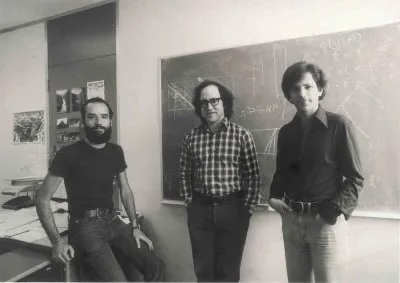
\includegraphics[width=0.7\linewidth]{Grundlagen_Info/03_Kryptologie/Figures/rsa.jpg}
	\caption{Ron Rivest, Adi Shamir und Leonard Adleman, die Erfinder des \gls{RSA}-Verfahrens}
	\label{fig:rsa}
\end{figure}


\begin{myprocedure}[\gls{RSA}-Verschlüsselungsverfahren]\label{myprocedure:RSA}
	Das \gls{RSA}-Verfahren besteht aus folgenden Schritten:
\begin{enumerate}
	\item \textbf{Schlüsselerzeugung:}
	      \begin{itemize}
		      \item Wählen Sie zwei (möglichst grosse) Primzahlen \( p \) und \( q \).
		      \item Berechnen Sie das \gls{RSA}-Modul \( n = p \cdot q \).
		      \item Berechnen Sie die Eulersche Funktion \( \varphi(n) = (p-1)(q-1) \).
		      \item Wählen Sie den \textit{Verschlüsslungsexponenten} \( e \), so dass dieser teilerfremd zu \( \varphi(n) \) und kleiner als $\varphi(n)$ ist. Dies bedeutet, dass der \gls{GGT} von $e$ und $\varphi(n)$ 1 ist ($\operatorname{ggT}(e, \varphi(n)) = 1$).
		      \item Berechnen Sie den \textit{Entschlüsslungexponenten} \( d \), so dass \( (e \cdot d) \mod \varphi(n) = 1  \) (privater Schlüssel). Dies bedeutet, dass, wenn man $d$ mit $e$ multipliziert und dieses Produkt Modulo $\varphi(n)$ rechnet, man die Zahl 1 erhält.
		      \item Die Zahlen $p$, $q$ und $\varphi(n)$ werden nun nicht mehr benötigt und können gelöscht werden.
	      \end{itemize}
	\item \textbf{Verschlüsselung:}
	      \begin{itemize}
		      \item Der Absender verschlüsselt eine \textbf{Klartext-Nachricht} \( \mathbf{m} \) (als Zahl) mit dem \textbf{öffentlichen Schlüssel} \( \mathbf{(e, n)} \):
		            \[
			            c = \mathbf{m}^e \mod n
		            \]
		      \item Das Ergebnis \( c \) ist der Kryptotext.
	      \end{itemize}
	\item \textbf{Entschlüsselung:}
	      \begin{itemize}
		      \item Der Empfänger entschlüsselt die \textbf{verschlüsselte Nachricht} \( \mathbf{c} \) mit dem \textbf{privaten Schlüssel} \( \mathbf{(d, n)} \):
		            \[
			            \mathbf{m} = c^d \mod n
		            \]
		      \item Das Ergebnis \( \mathbf{m} \) ist die ursprüngliche Nachricht.
	      \end{itemize}
\end{enumerate}
\end{myprocedure}

\begin{myexample}
Um \gls{RSA} besser zu verstehen, rechnen wir ein einfaches Beispiel mit kleinen Zahlen durch:
\begin{enumerate}
	\item Wir wählen zwei (für diese Übung kleine) Primzahlen aus, \( p = 3 \) und \( q = 11 \). Daraus folgt:
	      \begin{align*}
		      n & = p \cdot q  \\
		        & = 3 \cdot 11 \\
		        & = 33
	      \end{align*}
	      \begin{align*}
		      \varphi(n) & = (p-1)(q-1) \\
		                 & = 2 \cdot 10 \\
		                 & = 20
	      \end{align*}
	\item Wir wählen \( e = 3 \), da \( \operatorname{ggT}(3, 20) = 1 \).
	\item Wir berechnen \( d \), so dass \( (e \cdot d) \mod \varphi(n) = 1  \) ergibt:
	      \[
		      (d \cdot 3) \mod 20 = 1  \quad \rightarrow \quad d = 7.
	      \]
	\item Der öffentliche Schlüssel ist \( (e, n) = (3, 33) \), der private Schlüssel \( (d, n) = (7, 33) \).
\end{enumerate}

\textbf{Verschlüsselung:} Die Nachricht sei das Wort ``Code'', welches wir darstellen durch die Position der Buchstaben im Alphabet \( m = 3, 15, 4, 5 \). Berechne für jeden Buchstaben (hier nur für ``C'', also 3, gezeigt):
\begin{align*}
	c & = m^e \mod n  \\
	  & = 3^3 \mod 33 \\
	  & = 27 \mod 33  \\
	  & = 27.
\end{align*}


Der erste Buchstabe des Kryptotext wird also verschlüsselt als \( c = 27\).

\textbf{Entschlüsselung:}
\begin{align*}
	m & = c^d \mod n     \\
	  & = 27^{7} \mod 33 \\
	  & = 3
\end{align*}

Daraus ergibt sich \( m = 3 \), also die ursprüngliche Nachricht.
\end{myexample}


\begin{myexercise}\label{myexercise:rsa}
	Alice möchte eine Nachricht an Bob mit \gls{RSA} verschlüsseln. Bob wählt die Hilfs-Primzahlen \( p = 5 \) und \( q = 7 \). Generieren Sie den öffentlichen Schlüssel ($e, n$) und den privaten Schlüssel ($d, n$) von Bob, indem Sie folgende Schritte ausführen:
	\begin{enumerate}
		\item Berechnen Sie \( n \) und \( \varphi(n) \).
		\item Sie wählen $e$ und $d$ aus.
	\end{enumerate}

	Verschlüsseln Sie nun die Nachricht \( m = 9 \) mit dem öffentlichen Schlüssel \( (e, n) \).

	Entschlüsseln Sie danach die verschlüsselte Nachricht \( c \) wieder mit dem privaten Schlüssel \( (d, n) \).
	\begin{myanswer}
		\begin{enumerate}
			\item \( n = p \cdot q = 5 \cdot 7 = 35 \), \( \varphi(n) = (p-1)(q-1) = 4 \cdot 6 = 24 \).
			\item Für $e$ können wir beispielsweise 5 wählen, da 5 teilerfremd mit 24 ist.
			\item \( (5 \cdot d) \mod 24 = 1\). Dies finden wir beispielsweise mit \( d = 5 \).
			\item Verschlüsselung:
			      \begin{align*}
				      c & = m^e\mod n   \\
				        & = 9^5 \mod 35 \\
				        & = 4
			      \end{align*}.
			\item Entschlüsselung:
			      \begin{align*}
				      m & = c^d\mod n    \\
				        & =4^{5} \mod 35 \\
				        & = 9
			      \end{align*}
		\end{enumerate}
	\end{myanswer}
\end{myexercise}

\begin{myexercise}
	Ist die Wahl von \( p \) und \( q \) im obigen Beispiel sinnvoll? Begründen Sie Ihre Antwort.
	\begin{myanswer}
		Nein, die Wahl von \( p \) und \( q \) ist nicht sinnvoll, da beide Primzahlen zu klein sind. In der Praxis sollten \( p \) und \( q \) jeweils mindestens 2048 Bit lang sein, um eine ausreichende Sicherheit zu gewährleisten. Ansonsten kann es, wie im vorliegenden Beispiel, vorkommen, dass der private Schlüssel leicht durch Faktorisierung von \( n \) berechnet werden kann, oder dass der private Schlüssel sogar gleich dem öffentlichen Schlüssel ist (wie in diesem Beispiel, wo \( d = e = 5 \)).
	\end{myanswer}
\end{myexercise}

\begin{mychallenge}
	Wählen Sie zwei Primzahlen \( p \) und \( q \) mit jeweils mindestens 3 Ziffern. Generieren Sie den öffentlichen und privaten Schlüssel. Verschlüsseln Sie eine Nachricht Ihrer Wahl und entschlüsseln Sie diese wieder. Verwenden Sie Python, um die Berechnungen durchzuführen.

	Die Zahl $d$ kann in Python folgendermassen berechnet werden:

	Eine Liste der ersten 1000 Primzahlen finden Sie hier: \url{https://en.wikipedia.org/wiki/List_of_prime_numbers}
	\begin{lstlisting}
d = pow(e, -1, phi_n)
	\end{lstlisting}
	\begin{myanswer}
		Beispiel mit \( p = 101 \) und \( q = 113 \):
		\lstinputlisting{Grundlagen_Info/03_Kryptologie/Python package/encryption/rsa_simple.py}
	\end{myanswer}
\end{mychallenge}

\subsection{Digitale Signaturen mit \texorpdfstring{\acrshort{RSA}}{RSA}}
Neben der Verschlüsselung von Nachrichten kann das \gls{RSA}-Verfahren auch zur Erstellung digitaler Signaturen verwendet werden. Digitale Signaturen dienen dazu, die Authentizität und Integrität einer Nachricht zu gewährleisten. Hierbei wird die Nachricht mit dem privaten Schlüssel des Absenders signiert, sodass der Empfänger die Signatur mit dem öffentlichen Schlüssel des Absenders überprüfen kann.

\begin{myprocedure}[Digitale Signaturen mit \gls{RSA}]
	Die Erstellung und Überprüfung digitaler Signaturen mit dem \gls{RSA}-Verfahren erfolgt in folgenden Schritten:
\begin{enumerate}
	\item \textbf{Signaturerstellung:}
	      \begin{itemize}
		      \item Der Absender erstellt eine \textbf{Nachricht} \( \mathbf{m} \).
		      \item Er berechnet den \textbf{Hashwert} \( H(m) \) der Nachricht \( m \) mithilfe einer kryptographischen Hashfunktion (z.B. SHA-256).
		      \item Der Absender signiert den Hashwert mit seinem \textbf{privaten Schlüssel} \( \mathbf{(d, n)} \):
		            \[
			            s = H(m)^d \mod n
		            \]
		      \item Das Ergebnis \( s \) ist die digitale Signatur.
	      \end{itemize}
	\item \textbf{Signaturüberprüfung:}
	      \begin{itemize}
		      \item Der Empfänger erhält die Nachricht \( m \) und die Signatur \( s \).
		      \item Er berechnet den Hashwert \( H(m) \) der empfangenen Nachricht \( m \).
		      \item Der Empfänger überprüft die Signatur mit dem \textbf{öffentlichen Schlüssel} \( \mathbf{(e, n)} \) des Absenders:
		            \[
			            H'(m) = s^e \mod n
		            \]
		      \item Wenn \( H'(m) = H(m) \), ist die Signatur gültig, andernfalls ist sie ungültig.
	      \end{itemize}
\end{enumerate}
\end{myprocedure}

\begin{myexample}
	Angenommen, Alice möchte eine Nachricht \( m = 42 \) signieren. Sie verwendet ihren privaten Schlüssel \( (d, n) = (9677, 12317) \) und den öffentlichen Schlüssel \( (e, n) = (5, 12317) \).

	\textbf{Signaturerstellung:}
	\begin{align*}
		s & = H(m)^d \mod n \\
		  & = 42^{9677} \mod 12317 \\
		  & = 161
	\end{align*}

	Die digitale Signatur ist also \( s = 161 \).

	\textbf{Signaturüberprüfung:}
	\begin{align*}
		H'(m) & = s^e \mod n \\
		      & = 161^5 \mod 12317 \\
		      & = 42
	\end{align*}

	Da \( H'(m) = H(m) \), ist die Signatur gültig.
\end{myexample}

\begin{myexercise}
	Alice möchte die Nachricht \( m = 15 \) signieren. Ihr privater Schlüssel ist \( (d, n) = (7, 33) \) und ihr öffentlicher Schlüssel ist \( (e, n) = (3, 33) \).

	Erstellen Sie die digitale Signatur \( s \) für die Nachricht \( m \).

	Überprüfen Sie danach die Signatur mit dem öffentlichen Schlüssel.
	\begin{myanswer}
		\textbf{Signaturerstellung:}
		\begin{align*}
			s & = H(m)^d \mod n \\
			  & = 15^{7} \mod 33 \\
			  & = 27
		\end{align*}

		Die digitale Signatur ist also \( s = 27 \).

		\textbf{Signaturüberprüfung:}
		\begin{align*}
			H'(m) & = s^e \mod n \\
			      & = 27^3 \mod 33 \\
			      & = 15
		\end{align*}

		Da \( H'(m) = H(m) \), ist die Signatur gültig.
	\end{myanswer}
\end{myexercise}